\documentclass[final,5p,times,authoryear]{elsarticle}
\usepackage{amssymb}
\usepackage{amsmath}
\usepackage{multicol}
\usepackage{booktabs,array,float,xcolor,graphicx,tikz,adjustbox}
\usetikzlibrary{positioning,arrows.meta,shapes.geometric}
\newcommand{\todo}[1]{\textcolor{red}{[#1]}}
\newcommand{\KL}{\mathrm{KL}}
\emergencystretch=2em
\journal{Applied Soft Computing}

\begin{document}

\begin{frontmatter}

\title{Bayesian Network Structure Learning and Prior Selection Under Class Imbalance: A Controlled Study of Distribution Approximation and Fraud Detection}

\author{Mandisa N.\ Mashinini\\[3pt]\normalfont\small Supervised by Ritesh Ajoodha}
\affiliation{organization={School of Computer Science and Applied Mathematics, University of the Witwatersrand},
            city={Johannesburg},
            country={South Africa}}

\begin{abstract}
Fraud is rare, so probabilistic models of transactions must be learned from few positive cases. We studied Bayesian network learning for imbalanced fraud data in synthetic worlds whose data-generating network was known exactly, so that Kullback--Leibler (KL) divergence, F1 and the area under the ROC curve (AUROC) could be computed exactly, and we checked the main findings on a second synthetic mechanism and on real credit-card data. A network learned with Hill Climbing and the Bayesian information criterion (BIC) approximated the true distribution only from about 20,000 training rows (0.5\% fraud). A direct test and a trace of the search itself provide evidence that likelihood gains too small relative to the BIC complexity penalty are a major reason the fraud variable was not linked at small sample sizes: the gain from a true fraud edge grew with the number of fraud rows but stayed below the penalty until roughly 20,000 to 50,000 rows, and detection stayed at chance in every world where the variable was unlinked. With the true structure fixed, any prior was far closer to the truth than maximum likelihood (MLE) when data were scarce. A prior on the fraud rate also beat plain smoothing on both KL and detection when the smoothing of all other variables was held identical, but only while few fraud rows were available for each combination of the variables that the fraud label depends on: in the tested synthetic settings the average AUROC gain was largest below one such row, small between one and three, and negligible above about ten, a base rate estimated from a separate sample worked as well as the true rate, and a strong prior centred on a rate ten times too high was harmful. Learned graphs gave the fraud variable few parents, which left the prior with little to act on: with Hill Climbing it made no measurable difference in synthetic or real data, whereas naive Bayes and tree-augmented structures detected fraud on real data from a handful of fraud cases using ordinary smoothing alone. We propose exploratory selection guidelines based on fraud observations per parent configuration and prior strength; the numerical thresholds require further validation.
\end{abstract}



\begin{keyword}
Bayesian networks \sep Structure learning \sep Dirichlet priors \sep Class imbalance \sep Fraud detection \sep Kullback--Leibler divergence
\end{keyword}

\end{frontmatter}

\section{Introduction}
Fraud is rare. In card and mobile-money data, only a tiny fraction of transactions are fraudulent, so a model that learns from past transactions sees very few examples of the thing it is meant to find. Most fraud research trains classifiers that label each transaction as fraudulent or legitimate. This study takes a different route, using a Bayesian network: a model that describes how the transaction details (such as the type and amount) depend on one another and on whether fraud occurred. Its dependencies can be inspected, which makes its predictions easier to explain, and such models have been used against fraud for decades.

A Bayesian network must be learned from data in two steps: first the pattern of dependencies (its structure), then the probabilities that go with it. Rarity makes both steps hard. When fraud cases are few, many combinations of transaction details contain no fraud at all, and the model has little to base a probability on. The usual remedy is to start from a small amount of assumed prior information. The common choices of prior assume, without saying so, that fraud and legitimate transactions are about equally likely, which is far from the truth.

In real data the true distribution is never known, so it is impossible to say how close a learned model is to the truth. We therefore built artificial transaction worlds whose true distribution we know exactly. In each world we trained models on samples of different sizes and compared them with the truth, both in how closely they reproduce the true distribution and in how well they detect fraud. Because artificial worlds can flatter the methods that built them, we repeated the key comparisons with a second, differently constructed artificial mechanism and on a public set of real card transactions.

This study makes three contributions. First, it gives an exact evaluation of learned Bayesian networks against a known truth when fraud is rare, separating how closely a model reproduces the true distribution from how well it detects fraud. Second, it shows that the benefit of telling the model the fraud rate in advance is closely tracked by a single quantity, the number of fraud cases available for each combination of the variables that the fraud label depends on, and it turns this into exploratory guidelines for when such a prior may be preferred, how strong it should be and what to do instead. Third, it shows that the fraud-rate prior and structure learning compete as remedies for the same shortage of fraud cases, so that when the structure must also be learned the choice of structure matters more than the choice of prior; this was confirmed on a second artificial mechanism and on real data.

\section{Background and Related Work}\label{sec:related}
\subsection{Bayesian networks and probabilistic modelling}
Bayesian networks make the dependencies among transaction variables explicit. A Bayesian network over discrete variables $x_1,\dots,x_d$ with directed acyclic graph $G$ and parameters $\theta$ factorizes the joint distribution as a product of conditional distributions of each variable given its parents \citep{koller2009}. The factorization $P(x)=\prod_i P(x_i\mid \mathrm{pa}_i)$ means that learning reduces to estimating one conditional probability table per node, whose size grows exponentially with the number of parents; for a node with $q$ parent configurations and $r$ states there are $q(r-1)$ free parameters. Each prediction can be traced to these tables. Naive Bayes and tree-augmented networks are the best-known Bayesian-network classifiers \citep{friedman1997}.

\subsection{Structure learning: Hill Climbing and BIC}
Learning a network's structure from data is difficult and only partly identifiable. Score-based learning searches for a graph that maximizes a score such as BIC \citep{schwarz1978,cooper1992,heckerman1995}. The problem is NP-hard in general \citep{chickering1996}, so greedy search such as Hill Climbing is used: starting from a graph (here the empty one), it repeatedly applies the single edge addition, deletion or reversal that most increases the score, subject to acyclicity and a parent limit, and stops at a local optimum. The score decomposes over nodes, which makes each move cheap to evaluate. BIC is a large-sample approximation to the log marginal likelihood, whereas Bayesian Dirichlet scores such as K2 and BDeu use the prior directly \citep{cooper1992,heckerman1995}. The choice of score is not neutral: with BDeu, the best-scoring structure was shown to be highly sensitive to the equivalent sample size that sets the prior strength, for which there is no generally accepted rule \citep{silander2007}. BIC has no such parameter, but with a rare class the likelihood gain from adding a parent of the fraud node can be smaller than BIC's complexity penalty, so a real dependence on fraud can be left out of the learned graph; we examine this directly in Section~\ref{sec:edges}. Crucially, observational data identify a graph only up to Markov equivalence: graphs with the same skeleton and the same v-structures represent the same distribution \citep{verma1990,spirtes2000,chickering2002}. Exact recovery of the true arrows is therefore not an appropriate goal; what matters is how closely the learned model approximates the distribution. We adopt this view in RQ1.

\subsection{Parameter estimation: MLE and Dirichlet priors}
The choice of prior governs how a network's probabilities behave when data are scarce. With a Dirichlet prior, the posterior mean of a conditional probability is the observed count plus a pseudo-count, normalized \citep{heckerman1995,gelman2013,koller2009}. Because the Dirichlet is conjugate to the multinomial, the posterior is again Dirichlet, and the prior acts as imaginary observations: its total mass $\sum_v\alpha_v$ is the effective prior sample size, and its normalized form is the prior mean. For two outcomes the Dirichlet is a Beta distribution, so a prior on the fraud probability is Beta with mean $\alpha_{\text{fraud}}/(\alpha_{\text{fraud}}+\alpha_{\text{legit}})$. Maximum likelihood (MLE) is the case of zero pseudo-counts; it has no bias but high variance, and it assigns probability zero to any state not seen in training, which makes KL divergence infinite unless a floor is imposed. Jeffreys' prior adds 0.5 to every outcome \citep{jeffreys1946} and Laplace smoothing adds 1. Both are centred on equal probabilities. The influence of any prior fades as data accumulate \citep{gelman2013}; how fast, for a rare class, is one of our questions.

\subsection{Class imbalance in fraud detection}
Rare positives are the central difficulty of fraud detection. Reviews of the field describe a literature centred on supervised classification \citep{west2016,ali2022}. Learning from imbalanced data is surveyed by \citet{he2009}, and \citet{saito2015} show that precision--recall measures are more informative than the ROC curve when positives are rare. A related line of work concerns class probabilities rather than labels: undersampling the majority class at rate $\beta$ inflates the estimated posterior probability of the minority class and requires a correction \citep{dalpozzolo2015}, calibrated probabilities improve cost-based fraud decisions \citep{correa2014}, and the effect of changing class priors on decisions is a basic result of cost-sensitive learning \citep{elkan2001}. Other imbalance strategies act on the data rather than on the probabilities: resampling the training set, for example by creating synthetic minority examples through interpolation \citep{chawla2002}, or by undersampling the majority class. These change what the model sees, whereas a prior changes how the model converts few observations into a probability. These works motivate our focus on how the assumed class prior enters probability estimation, and our choice to vary the fraud rate and sample size together under one protocol.

\subsection{Existing research and the remaining gap}
Bayesian networks have a long but mostly empirical record in fraud detection. Early applications include learning for fraud and uncollectible-debt detection \citep{ezawa1995}, a comparison of Bayesian and neural networks for credit card fraud \citep{maes2002}, and a comparison of decision trees, neural networks and Bayesian belief networks for fraudulent financial statements \citep{kirkos2007}. Such studies report predictive scores on real data, where the distance from the true distribution cannot be measured. Public synthetic datasets such as PaySim \citep{lopez2016} are generated by agent-based simulation, so although they are convenient and shareable, their true dependency structure is not available either. Comparing a learned graph with a randomly generated graph shows only that the learned model differs from noise, not how close it is to the truth. More recent work continues to apply Bayesian methods to financial risk and fraud, for example Bayesian logistic regression inside a wider risk-forecasting pipeline \citep{almamun2025}, and to the small-sample parameter problem for Bayesian networks, for example constrained adjusted maximum a posteriori estimation \citep{camap2021}. Neither compares priors against a known truth under rare-class sampling. These studies leave open how the implicit equal-class belief of symmetric priors affects probability estimation when one class is as rare as 0.5\% or less, and how the answer changes with the fraud rate and the amount of data. Answering this requires a controlled comparison in which the true distribution is known, the fraud rate and sample size are varied together, and estimators are compared by both distributional closeness and detection, which is the aim of this study.

\section{Methodology and Experiments}
\subsection{Problem statement and technical purpose}\label{sec:problem}
On real or simulated fraud data the generating distribution is unknown, so a study can report predictive scores but cannot say how close the learned distribution is to the truth, or whether a change in F1 reflects better probabilities or an artefact of the decision threshold. Accuracy is known to mislead under imbalance \citep{he2009,saito2015}: a rule that always answers ``legitimate'' is 99.5\% accurate at a 0.5\% fraud rate and detects nothing. Widely used simulators such as PaySim \citep{lopez2016} are agent-based programs rather than Bayesian networks, so the true conditional distribution over their variables is not available in closed form.

Three questions are kept separate throughout. Structure and distribution quality: how closely the learned model reproduces the true distribution (KL divergence), and whether the fraud node is connected at all. Predictive performance: how well the model ranks and detects fraud (F1 and AUROC). Prior sensitivity: how strength, the assumed base rate and the fraud rate change the other two. Because the true distribution is known, no random-graph baseline is needed; the empty graph (no dependencies) and the true graph bound what a learned structure can achieve.

The purpose of the experiments is to measure, against a known truth, how well a Bayesian network can be learned from imbalanced data and which parameter estimator is preferable under which conditions. Two research questions follow.

RQ1: how well can a Bayesian network learned with Hill Climbing and the Bayesian information criterion (BIC) approximate the true data-generating distribution under severe class imbalance, as the amount of training data grows?

RQ2: how do sample size, prior choice (maximum likelihood, Jeffreys, Laplace and a fraud-base-rate-informed prior), prior strength and class imbalance (the true fraud rate) affect how closely the estimated distribution matches the true one (measured by KL divergence) and fraud detection performance (F1, with AUROC as a secondary measure)?

Because observational data identify a graph only up to Markov equivalence, RQ1 does not ask whether the true arrows are recovered; it asks how closely the learned model approximates the ground-truth probability distribution, as measured by KL divergence. The objectives are (i) to measure that approximation as a learning curve, (ii) to isolate the effect of parameter estimation by fixing the true structure, and (iii) to map which estimator is preferable under which tested conditions.

\subsection{Experimental framework}
Fig.~\ref{fig:design} summarizes the design. A world with a known network is built, data are sampled and the truth is hidden; a model is learned from the data and then compared with the truth. RQ1 uses structures learned by Hill Climbing; RQ2 gives every estimator the true structure, so that differences come only from how the probabilities are estimated, not from structure errors.

\begin{figure}[H]
\centering
\begin{adjustbox}{max width=\linewidth}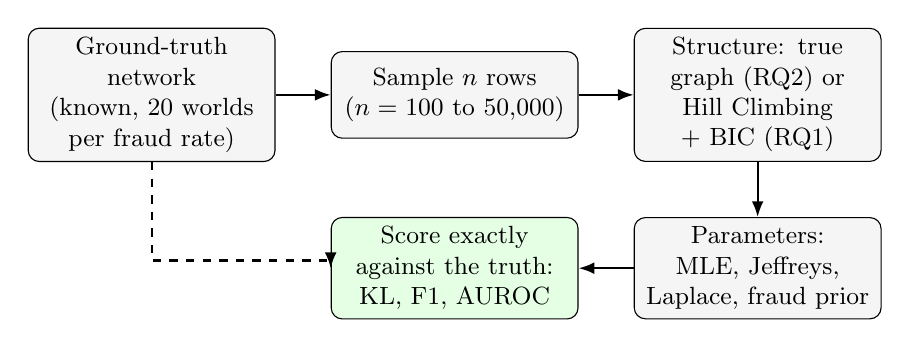
\begin{tikzpicture}[node distance=7mm,
  box/.style={draw,rounded corners,align=center,minimum height=11mm,text width=2.9cm,font=\small,fill=gray!8},
  arr/.style={-{Latex[length=2mm]},thick}]
\node[box] (a) {Ground-truth network\\(known, 20 worlds per fraud rate)};
\node[box,right=of a] (b) {Sample $n$ rows\\($n=100$ to $50{,}000$)};
\node[box,right=of b] (c) {Structure: true graph (RQ2) or Hill Climbing + BIC (RQ1)};
\node[box,below=of c] (d) {Parameters: MLE, Jeffreys, Laplace, fraud prior};
\node[box,left=of d,fill=green!10] (e) {Score exactly against the truth: KL, F1, AUROC};
\draw[arr] (a)--(b); \draw[arr] (b)--(c); \draw[arr] (c)--(d); \draw[arr] (d)--(e);
\draw[arr,dashed] (a.south) -- ++(0,-1.25) -| (e.west);
\end{tikzpicture}\end{adjustbox}
\caption{Experimental design. The dashed arrow shows that the truth is used only for scoring.}\label{fig:design}
\end{figure}

\subsection{Synthetic ground-truth Bayesian network generation}
Each world is a Bayesian network over the nine variables in Table~\ref{tab:vars}, which mirror the variables of the PaySim simulator \citep{lopez2016}. All variables are natively discrete (five states for the transaction type and for each balance, amount and balance-error variable, two for the fraud label). Variables are arranged in five tiers, and a directed edge may only go from an earlier tier to a later one, so the graph is acyclic by construction. For each node, each candidate parent in an earlier tier is retained with probability 0.5, up to a maximum of three parents; \texttt{isFraud} is forced to have at least one parent. Each row of every non-fraud conditional table is drawn from a symmetric Dirichlet distribution with concentration 2 per state. For \texttt{isFraud}, the fraud probability of every parent configuration is drawn from a Beta distribution with mean equal to the target fraud rate and concentration $a+b=40$, so that fraud is rare overall but varies across configurations. At the default 0.5\% rate the 20 true graphs have 10 to 16 edges (mean 13.9), \texttt{isFraud} has one to three parents (mean 2.7), and the realised marginal fraud rate has mean 0.51\% (range 0.25\% to 1.05\%).

\begin{table}[H]
\centering\small
\begin{adjustbox}{max width=\linewidth}
\begin{tabular}{lccl}\toprule
Variable & States & Tier & Allowed parents\\\midrule
type, oldbalanceOrg, oldbalanceDest & 5 & 0 & none (roots)\\
amount & 5 & 1 & tier 0\\
newbalanceOrig, newbalanceDest & 5 & 2 & tiers 0--1\\
delta\_orig, delta\_dest & 5 & 3 & tiers 0--2\\
isFraud & 2 & 4 & tiers 0--3 (at least one parent)\\\bottomrule
\end{tabular}
\end{adjustbox}
\caption{Variables of the ground-truth worlds. A node may take parents only from earlier tiers.}\label{tab:vars}
\end{table}

\subsection{Fraud prevalence and sample-size conditions}
For RQ2 we built worlds at five target fraud rates: 0.1\%, 0.5\%, 2\%, 5\% and 10\%. The same 20 seeds (42 to 61) and the same nine nested sample sizes ($n=100$, 200, 500, 1,000, 2,000, 5,000, 10,000, 20,000, 50,000) were used at every rate, so differences between rates are not caused by different seeds or sample sizes. A given seed yields the same graph at every rate; only the fraud table, and hence the sampled data, changes. Table~\ref{tab:worlds} shows the realised conditions. One property of this design matters for interpretation: because the Beta concentration is held at 40, a low target rate gives very uneven fraud probabilities across parent configurations (fraud is concentrated in a few configurations, hence more predictable), whereas a high target rate gives nearly even ones. The best achievable AUROC therefore falls from 0.96 at 0.1\% to 0.64 at 10\%. Fraud rate and predictability are thus confounded in these worlds, and we return to this in Section~\ref{sec:limits}. To separate the two, we also built controlled worlds in which the Beta concentration was chosen separately for each fraud rate (by bisection on eight worlds) so that the mean best AUROC is about 0.80 at every rate (Section~\ref{sec:ctrl}); the same seeds, sample sizes and estimators were used.

\begin{table}[H]
\centering\small
\begin{adjustbox}{max width=\linewidth}\begin{tabular}{rcrrrrr}\toprule
Target rate & Realised rate (min--max) & Fraud rows at $n{=}100$ & $n{=}1{,}000$ & $n{=}10{,}000$ & Best F1 & Best AUROC\\\midrule
0.1\% & 0.09\% (0.01--0.22\%) & 0.2 & 1 & 9 & 0.054 & 0.963\\
0.5\% & 0.51\% (0.25--1.05\%) & 0.7 & 6 & 54 & 0.082 & 0.888\\
2\% & 2.01\% (1.51--2.80\%) & 2.0 & 21 & 205 & 0.120 & 0.768\\
5\% & 4.95\% (3.81--5.84\%) & 5.3 & 50 & 497 & 0.163 & 0.684\\
10\% & 9.94\% (8.44--10.68\%) & 10.2 & 102 & 1002 & 0.234 & 0.640\\
\bottomrule\end{tabular}\end{adjustbox}
\caption{Fraud-rate conditions (20 worlds per rate). Realised rate: marginal $P(\text{fraud})$ of the worlds. Fraud rows: mean number of fraud rows in a training sample of the stated size. Best F1 and AUROC: values achieved by the true model (mean over worlds).}\label{tab:worlds}
\end{table}

\subsection{Structure-learning experiment (RQ1)}
Structures are learned with the Hill Climbing search of pgmpy 1.1.2 \citep{ankan2015} with the BIC score \citep{schwarz1978}, a maximum of four parents per node, and a single run from the empty graph (no restarts). BIC rewards the fit of the maximum-likelihood parameters and penalizes the number of free parameters in proportion to $\log n$. Training sets are nested prefixes of one sample per world, so that each curve is a function of $n$ alone. Learned networks use Laplace parameters, with the true structure and an empty graph as references. RQ1 was run at the default 0.5\% fraud rate (20 worlds).

\subsection{Parameter-learning experiments (RQ2)}
Four estimators are applied to the true structure (Table~\ref{tab:est}). Each estimator adds pseudo-counts $\alpha_v$ to the observed count $N_{v,\mathrm{pa}}$ of every state $v$ under each parent configuration $\mathrm{pa}$ and normalizes, which is the standard Dirichlet posterior mean. MLE is $\alpha_v=0$. Our modification is the fraud-informed prior, which acts on the fraud node only. For strength $s$ and assumed base rate $r$, the pseudo-counts for each parent configuration of \texttt{isFraud} are
\begin{equation}
\alpha_{\text{fraud}}=s\,r,\qquad \alpha_{\text{legit}}=s\,(1-r),
\end{equation}
that is, a Beta$(sr,\,s(1-r))$ prior centred on $r$ and worth $s$ imaginary samples; all other nodes use the Jeffreys prior. The base rate is fixed and is never computed from the training sample, because a prior set from the data would not be independent of them. Ordinary MLE is undefined for a parent configuration with no training rows. As an implementation convention, such a configuration receives a uniform distribution under MLE and the prior mean under the other estimators. The convention matters for MLE at small $n$, so we also tried the alternative of giving the configuration the node's overall sample frequencies (Section~\ref{sec:robust}).

\begin{table}[H]
\centering\small
\begin{adjustbox}{max width=\linewidth}
\begin{tabular}{lll}\toprule
Estimator & Pseudo-counts & Prior mean of $P(\text{fraud})$\\\midrule
MLE & 0 & observed frequency (unseen configuration: uniform)\\
Jeffreys & 0.5 on every outcome & 0.5 (equal probabilities)\\
Laplace & 1 on every outcome & 0.5 (equal probabilities)\\
Fraud prior (FP$s$) & isFraud: $sr$, $s(1-r)$; others 0.5 & $r$\\\bottomrule
\end{tabular}
\end{adjustbox}
\caption{Parameter estimators compared. $s$ is the strength (imaginary samples) and $r$ the assumed base rate.}\label{tab:est}
\end{table}

\subsection{Prior strengths and misspecification}
Two versions of the fraud prior were used at every fraud rate, with strengths $s\in\{2,10,50,200\}$. In the true-rate version ($\mathrm{FP}_{\text{true}}$) $r$ equals the world's target rate, which is the best case in which the base rate is known. In the fixed-guess version ($\mathrm{FP}_{\text{fix}}$) $r=0.5\%$ at every rate, a misspecified belief at all rates except 0.5\%. The true-rate version is a best-case benchmark that uses the generating rate; Section~\ref{sec:rate} compares it with rates estimated from a separate historical sample or from the training sample, and with deliberately wrong rates. A separate experiment at the 0.5\% rate crossed strength $s\in\{1,10,50,200,500\}$ with believed base rates of 0.05\%, 0.5\%, 2\%, 5\% and 50\%.

\subsection{Evaluation metrics: KL, F1 and AUROC}
The closeness of an estimated distribution $\hat P$ to the truth $P$ is measured by a floored Kullback--Leibler divergence \citep{kullback1951}. Because MLE can assign probability zero to a state that has positive true probability, which would make the ordinary divergence infinite, every estimated conditional probability is floored at $10^{-4}$ before the logarithm is taken:
\begin{multline}
\KL_{\text{floor}}(P\,\|\,\hat P)=\sum_x P(x)\,\Big[\log P(x)\\-\sum_{i}\log\max\{\hat P(x_i\mid \mathrm{pa}_i),10^{-4}\}\Big].
\end{multline}
The floored model is not a normalized distribution, so this quantity is not the ordinary KL divergence; it equals it only when no estimated conditional probability falls below the floor. We report it as a distance measure whose value depends on the floor for MLE, and test that dependence in Table~\ref{tab:floor}. Because each world has only $5^8\times 2=781{,}250$ joint states, we enumerate all of them, so this sum is exact; the floor mainly affects MLE. A fitted model scores each state with the posterior probability of fraud given all other variables. Treating each state as a row weighted by its true probability gives the population F1 (maximised over decision thresholds, which we call the oracle-threshold F1) and AUROC of the model, that is, the values an infinitely large test set would give. The fitted probabilities were checked against an independent pgmpy implementation (maximum difference $10^{-16}$), the exact KL against a Monte Carlo estimate (within two standard errors), and the exact F1 and AUROC against scikit-learn \citep{pedregosa2011} (maximum difference $10^{-17}$). The oracle-threshold F1 is optimistic because the threshold uses knowledge of the true distribution, so it is not a real-world estimate. We therefore also report AUROC, which needs no threshold, and, for the 0.5\% experiment, an F1 in which the threshold is chosen on a separate validation sample drawn from the same world with the same size as the training sample (Table~\ref{tab:val}). Accuracy is not used, for the reason given in Section~\ref{sec:problem}. As a check that KL separates close from far, in ten independent pairs of worlds the KL of a structure learned from a world's own data averaged 0.071 (SD 0.042), against 3.858 (SD 0.591) for a structure learned from the other world; the per-pair ratio ranged from 26 to 137 with no overlap.

\subsection{Statistical analysis and reproducibility}
Curves show means over worlds with 95\% $t$ confidence intervals (medians and inter-quartile ranges where stated). Estimators are compared by paired differences within each world, using Wilcoxon signed-rank tests \citep{wilcoxon1945}. For the learning-curve experiment at 0.5\% fraud, $p$-values are Holm-corrected \citep{holm1979} across 108 comparisons and reported with 95\% confidence intervals and the paired effect size $d_z$ (mean difference divided by its standard deviation). For the fraud-rate maps (Figs.~\ref{fig:map} and~\ref{fig:mapc}) each cell contains three paired Wilcoxon tests of $\mathrm{FP}_{\text{true}}$ with $s=50$, one against each of MLE, Jeffreys and Laplace, so no comparator is chosen from the same data. All 270 tests of an experiment (45 conditions, three comparators, two metrics) are Holm-corrected together. A cell is marked as favouring the fraud prior only if it is significantly better than all three, and as favouring a standard method if at least one of them is significantly better. Tests treat the 20 worlds as independent, and the analyses remain exploratory in the sense that they cover one prior strength and one world generator. The Holm-corrected analyses (the 108 comparisons at 0.5\% fraud and the two 270-test maps) are the main analyses of the study. Everything else is exploratory: the matched-smoothing, rate-source, $k$-measure, structure, real-data and BIC analyses. For the exploratory analyses that support a main claim we report effect sizes with 95\% bootstrap intervals that resample worlds, and uncorrected $p$-values only as a guide. The same 20 worlds are reused across sample sizes and across experiments, so results at different sizes and in different tables are not independent evidence, and the intervals resample worlds, not runs. The synthetic data are generated from fixed random seeds (42 to 61) and one real data set is used (Section~\ref{sec:extra}); results regenerate with a fixed hash seed (\texttt{PYTHONHASHSEED=0}), which also fixes the tie-breaking of pgmpy's Hill Climbing; the outputs of the learning-curve, fraud-rate, learned-structure, second-generator and real-data experiments were regenerated from a clean environment with this setting (the first two reproduced the stored results exactly). The code, result files and report source are provided in the repository submitted with this report, whose README maps each table and figure to the script that produces it.

\subsection{Learned structures, a second mechanism and real data}\label{sec:extra}
Three further experiments tested whether the conclusions depend on the true structure, on the generator, or on synthetic data. In the first, the structure was learned rather than given. Besides Hill Climbing with BIC we learned naive Bayes, in which the fraud node is the parent of every other variable, and a tree-augmented network (TAN), a naive Bayes with a tree added among the other variables \citep{friedman1997}. These structures keep the fraud node at the root, so it has a single parent configuration. They were run in the original worlds at fraud rates of 0.5\% and 2\% (20 worlds, four sample sizes), with the same estimators as before.

In the second, the data came from a different mechanism, in which the observed variables are not generated by a sparse network. Each transaction first receives one of three latent classes. Given the class, the eight variables are drawn independently from skewed distributions. The fraud probability is then a logistic function of the variables, with an intercept solved so that the fraud rate is exact and a scale solved so that the best achievable AUROC is 0.80. The joint distribution is still enumerable, so all metrics remain exact, but no sparse network represents it. We learned three structures from this generator: Hill Climbing, naive Bayes, and a fixed structure in which the fraud node has the three most informative variables as parents (20 worlds, five fraud rates, five sample sizes).

In the third, we used the public credit-card fraud data of European card holders (284,807 transactions, 492 fraudulent, 0.17\%) released with \citet{dalpozzolo2015}. Its 28 numeric features are anonymised principal components, so the variables cannot be named. For each of 30 repeats we split the data 70/30 with the fraud rate preserved, selected eight features by mutual information with the label on the training part, discretised them into up to five quantile bins, drew training samples of 1,000 to 60,000 rows (and the whole training part), and scored the held-out part by AUROC, average precision and log loss. There is no ground truth here, so KL cannot be computed. The fraud prior was centred on the training fraud rate, and a mis-centred prior (0.5\%) was also run.

Two further experiments tested explanations directly. To test why Hill Climbing misses fraud, we took the true parents of the fraud node in the original worlds at 0.5\% fraud (20 worlds, nine sample sizes up to 50,000, nested samples) and, for each true parent in turn, computed the change in log-likelihood, the BIC penalty $\tfrac12\ln n$ per extra parameter, and their difference when that single edge is added to a fraud node with no parents, which is the move a greedy search considers first. We also computed the same quantities for all true parents together. To check that this single-edge test describes what the search actually faces, we traced Hill Climbing step by step with our own implementation (empty start, add, remove and reverse moves, at most four parents, checked against pgmpy's search), recording at every step the accepted move and the best move involving the fraud node, in the same worlds and on the real data. To make the comparison of estimators fair, we added a fraud prior of strength 50 that uses Laplace smoothing on every non-fraud node, so that it differs from Laplace smoothing only in the fraud node (and the existing fraud prior differs from Jeffreys smoothing only in the fraud node). This was run in the original worlds at fraud rates of 0.5\% and 2\% (20 worlds, nine sizes, true structure). The rate of the fraud prior was also varied: the true world rate, a rate estimated on a separate historical sample of 1,000 or 10,000 rows from the same world, a rate estimated from the training sample itself (all Jeffreys-smoothed fractions), and rates ten times too low and ten times too high. Finally, because parent configurations occur at very different frequencies, we computed from the actual fraud counts per configuration of the fraud node the share of configurations with no fraud row, the probability mass of those configurations, the median count and a mass-weighted count, and compared how well each predicts the prior's gain.

To compare conditions across all these experiments we use the expected number of fraud rows per parent configuration of the fraud node,
\begin{equation}
k=\frac{n\,\pi}{q},
\end{equation}
where $n$ is the number of training rows, $\pi$ the fraud rate and $q$ the number of configurations of the fraud node's parents ($q=1$ if it has none). We also use $\varphi=s\,r_b/k$, the number of pseudo-fraud rows that a prior of strength $s$ and believed rate $r_b$ places in each configuration, relative to the number the data supply. To study strength, in the original worlds at 0.5\% fraud with the true structure (20 worlds, six sample sizes) we fitted the fraud prior with strengths $s$ from 1 to 500 and believed rates of 0.05\%, 0.5\%, 2\%, 5\% and 50\%, that is 0.1, 1, 4, 10 and 100 times the true rate. Gains are reported as the change in AUROC relative to Jeffreys smoothing, which smooths every non-fraud node exactly as the fraud prior does, and significance by paired Wilcoxon tests that are uncorrected for multiple testing and exploratory.
\section{Results and Discussion}
\subsection{RQ1: distribution approximation as sample size grows}
Fig.~\ref{fig:rq1} places the learned network between two references (all with Laplace parameters, 0.5\% fraud, 20 worlds). A model with no edges has a median KL of about 0.83 at any sample size. The learned network improves on it only gradually (median KL 0.72 at 500 samples and 0.50 at 5,000, against 0.60 and 0.13 for the true structure), and its AUROC stays near 0.5 until about 10,000 samples. Between 10,000 and 20,000 samples its median KL falls from 0.38 to 0.044, close to the true structure's 0.038, and at 50,000 samples it is 0.021 against 0.016. Progress was not monotone: in six of the 20 worlds (four of them by more than 0.05) the learned network was worse at 50,000 than at 20,000 samples, because greedy search settled on a differently oriented network that is not equivalent to the truth. In answer to RQ1, as the training sample size increased, the network learned by Hill Climbing with BIC became a closer approximation of the ground-truth distribution, as indicated by decreasing KL divergence, but it was close (median KL below 0.05) only from about 20,000 rows at this fraud rate. Below that size the learned distribution is barely closer to the truth than one that treats the variables as independent, so conclusions drawn from it about fraud should be treated with caution.

\begin{figure*}[t]
\centering
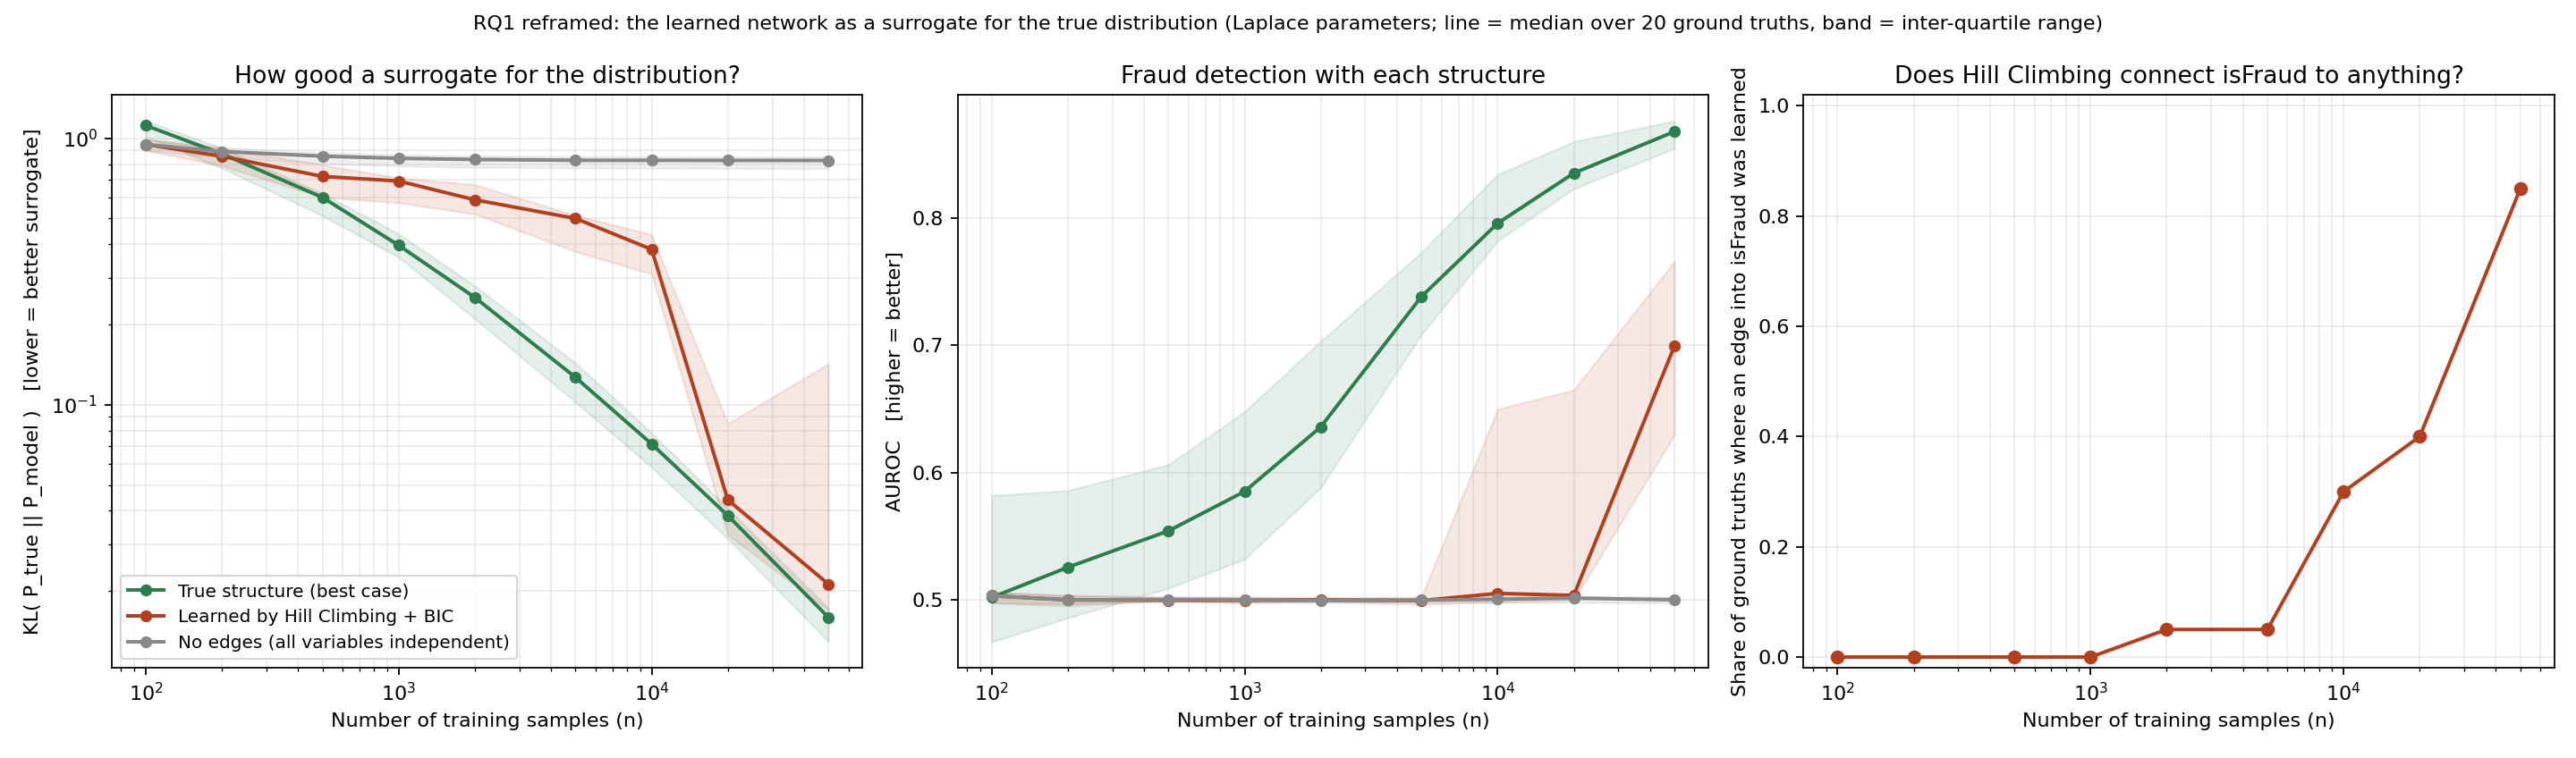
\includegraphics[width=0.78\textwidth]{figs/lc_rq1_surrogate.png}
\caption{Closeness of the learned network to the ground-truth distribution (Laplace parameters). Lines are medians over 20 worlds and bands the inter-quartile range. (a) KL divergence; (b) AUROC; (c) percentage of worlds in which an edge into \texttt{isFraud} was learned.}\label{fig:rq1}
\end{figure*}

\subsection{RQ1: fraud-edge recovery}\label{sec:edges}
In the first 15 worlds at 20,000 samples, Hill Climbing recovered edges with precision 0.698 (SD 0.199) and recall 0.622 (SD 0.154); the structural Hamming distance averaged 6.27 (SD 3.03). Recovery was uneven (Table~\ref{tab:edges}): edges outside \texttt{isFraud} were recovered in 120 of 163 cases (a case is one true edge in one world; 74\%; per-edge-type median 80\%, range 12\% to 100\%), whereas edges into \texttt{isFraud} were recovered in only 5 of 40 cases (12.5\%); \texttt{amount}$\to$\texttt{isFraud} and \texttt{type}$\to$\texttt{isFraud} were never found, and no individual fraud edge was recovered in more than 2 of the 8 worlds in which it was true. An edge into \texttt{isFraud} was learned in none of the 20 worlds up to 1,000 samples, in 5\% at 2,000 and 5,000, in 30\% at 10,000, 40\% at 20,000 and 85\% at 50,000 samples (Fig.~\ref{fig:rq1}c). In the five worlds where at least one true fraud parent was recovered, AUROC averaged 0.74; in the other ten it averaged 0.51, essentially chance. The fraud node is the hardest part of the structure to learn, so the learned network fails exactly where detection needs it; recovering the other edges well does not compensate.

\begin{table}[H]
\centering\small
\begin{adjustbox}{max width=\linewidth}
\begin{tabular}{lccc}\toprule
Edge & Worlds where true & Worlds recovered & Recovery\\\midrule
newbalanceDest $\to$ isFraud & 8 & 2 & 25\%\\
oldbalanceOrg $\to$ isFraud & 4 & 1 & 25\%\\
newbalanceOrig $\to$ isFraud & 4 & 1 & 25\%\\
delta\_orig $\to$ isFraud & 4 & 1 & 25\%\\
type $\to$ isFraud & 8 & 0 & 0\%\\
amount $\to$ isFraud & 6 & 0 & 0\%\\
oldbalanceDest $\to$ isFraud & 3 & 0 & 0\%\\
delta\_dest $\to$ isFraud & 3 & 0 & 0\%\\\bottomrule
\end{tabular}
\end{adjustbox}
\caption{Recovery of individual true edges by Hill Climbing (15 worlds, 20,000 samples): all edges into isFraud. Edges outside isFraud were recovered far more often (text).}\label{tab:edges}
\end{table}


\subsection{RQ2: MLE versus Bayesian priors for KL}
At 0.5\% fraud, with the true structure fixed, every prior was significantly closer to the truth than MLE at every size from 100 to 50,000 (Fig.~\ref{fig:kl}). MLE was 11.2 times further from the truth than the best prior at 100 samples, 4.7 times at 2,000, 2.0 times at 10,000 and still 1.24 times at 50,000. MLE's curve is steeper (log--log slope $-1.28$ for $n\ge1{,}000$, against $-0.83$ to $-0.87$ for the priors), so it starts far behind and catches up, but the gap had not closed within the range tested. Laplace and the fraud-informed prior were statistically indistinguishable except at 100 samples, where the fraud prior was closer (18 of 20 worlds, Holm-adjusted $p=0.002$). With rare events, smoothing is not optional: omitting it costs an order of magnitude in KL at small $n$, and choosing between the smoothed priors matters far less.

\begin{figure}[t]
\centering
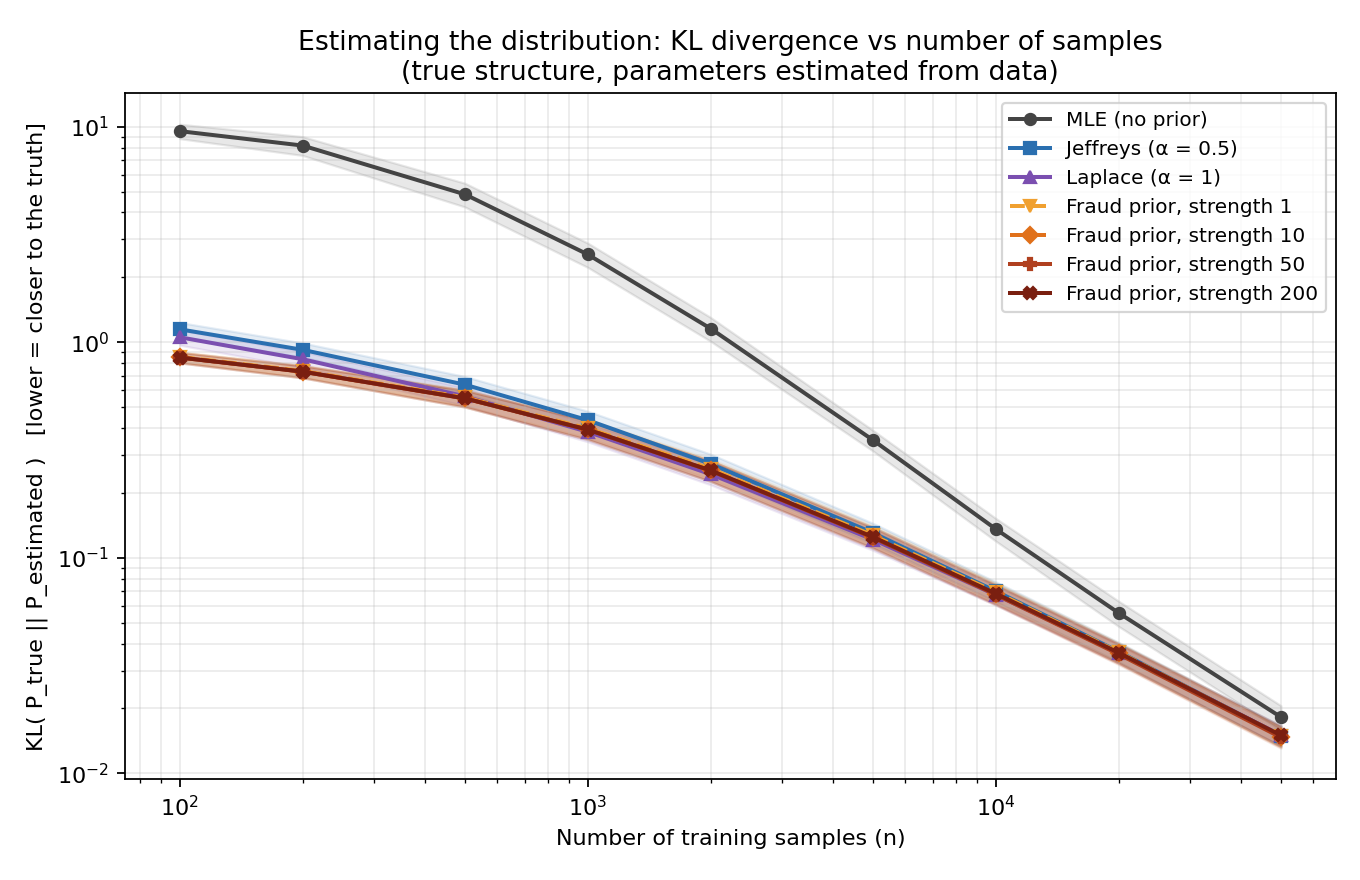
\includegraphics[width=\columnwidth]{figs/lc_kl_vs_n.png}
\caption{KL divergence from the true distribution against the number of training samples, with the true structure (0.5\% fraud; mean and 95\% confidence interval over 20 worlds; log axes; lower is better).}\label{fig:kl}
\end{figure}





\subsection{Robustness of the evaluation}\label{sec:robust}
Table~\ref{tab:floor} shows that the floor changes the KL of MLE a great deal at small $n$ (at 100 rows from 3.6 to 21 as the floor goes from $10^{-2}$ to $10^{-8}$), because MLE assigns zero to many conditional probabilities, whereas the KL of the smoothed estimators is the same to three decimals from $10^{-8}$ to $10^{-3}$. MLE remained further from the truth than every smoothed estimator at every floor, with the single exception of a near-tie at 50,000 rows with the largest floor. The conclusion that smoothing matters is robust to the floor, but the numerical size of MLE's divergence is not, and the value of about 9.5 at 100 rows should be read as specific to a floor of $10^{-4}$.

Giving unseen configurations the node's overall frequencies instead of a uniform distribution lowered MLE's KL only slightly (for example 9.37 against 9.54 at 100 rows) but raised its F1 at small $n$ (0.029 against 0.021 at 100 rows and 0.049 against 0.033 at 500). Part of the fraud prior's F1 advantage over MLE at a few hundred rows reflects the poor convention for unseen configurations, and the advantage shrinks when MLE is given a more sensible fallback.

With the threshold chosen on validation data (Table~\ref{tab:val}), F1 is lower for every estimator, as expected. The fraud prior still had a significantly higher F1 than Laplace from 500 to 20,000 rows (Wilcoxon, $p\le0.005$, uncorrected, 19 to 20 worlds). Against MLE the oracle-threshold advantage at 2,000 to 5,000 rows (0.003 to 0.005, $p\le0.024$) disappeared (differences of $-0.0003$ and 0.0, $p>0.3$); it remained at 500 rows (0.008, $p=0.008$). Oracle-threshold F1 overstates the benefit of the fraud prior relative to MLE; the benefit relative to Laplace is robust.

\begin{table}[H]
\centering\small
\begin{adjustbox}{max width=\linewidth}\begin{tabular}{rlccccc}\toprule
$n$ & Estimator & $10^{-2}$ & $10^{-3}$ & $10^{-4}$ & $10^{-6}$ & $10^{-8}$\\\midrule
100 & MLE (uniform for unseen) & 3.63 & 6.58 & 9.54 & 15.44 & 21.35\\
100 & MLE (marginal for unseen) & 3.47 & 6.42 & 9.37 & 15.28 & 21.19\\
100 & Laplace & 1.05 & 1.05 & 1.05 & 1.05 & 1.05\\
100 & Fraud prior $s=50$ & 0.844 & 0.850 & 0.850 & 0.850 & 0.850\\
2,000 & MLE (uniform for unseen) & 0.465 & 0.812 & 1.16 & 1.85 & 2.54\\
2,000 & MLE (marginal for unseen) & 0.464 & 0.810 & 1.16 & 1.85 & 2.54\\
2,000 & Laplace & 0.244 & 0.244 & 0.244 & 0.244 & 0.244\\
2,000 & Fraud prior $s=50$ & 0.250 & 0.254 & 0.254 & 0.254 & 0.254\\
\bottomrule\end{tabular}
\end{adjustbox}
\caption{Mean KL divergence at 0.5\% fraud (true structure, 20 worlds) for different probability floors (columns). MLE (uniform) is the convention used in the main experiments.}\label{tab:floor}
\end{table}

\begin{table}[H]
\centering\small
\begin{adjustbox}{max width=\linewidth}\begin{tabular}{rcccccc}\toprule
 & \multicolumn{2}{c}{MLE} & \multicolumn{2}{c}{Laplace} & \multicolumn{2}{c}{Fraud prior $s=50$}\\\cmidrule(lr){2-3}\cmidrule(lr){4-5}\cmidrule(lr){6-7}
$n$ & Oracle & Valid. & Oracle & Valid. & Oracle & Valid.\\\midrule
500 & 0.033 & 0.025 & 0.025 & 0.017 & 0.053 & 0.033\\
2,000 & 0.058 & 0.050 & 0.037 & 0.031 & 0.061 & 0.050\\
5,000 & 0.069 & 0.061 & 0.049 & 0.040 & 0.074 & 0.061\\
20,000 & 0.079 & 0.075 & 0.073 & 0.067 & 0.080 & 0.075\\
\bottomrule\end{tabular}
\end{adjustbox}
\caption{Mean F1 at 0.5\% fraud with the oracle threshold and with a threshold chosen on a separate validation sample of size $n$ (20 worlds; one world at $n=500$ had no fraud in its validation sample and is excluded from the validated column).}\label{tab:val}
\end{table}

\subsection{RQ2: F1 and AUROC comparisons}
At 0.5\% fraud the ranking of the estimators differs for detection (Fig.~\ref{fig:det}, Table~\ref{tab:f1}; differences are paired within worlds and Holm-corrected over 108 comparisons). The fraud-informed prior had a significantly higher AUROC than Laplace from 500 to 50,000 samples (gain 0.02 to 0.05 between 500 and 20,000 samples; paired $d_z$ 0.69 to 1.25) and a significantly higher F1 between 500 and 5,000 samples (gain 0.024 to 0.028, which roughly doubles F1 at 500 samples: 0.025 to 0.053). Jeffreys and Laplace were significantly worse than MLE on F1 at 2,000 and 5,000 samples. Compared with MLE, the fraud prior was significantly better on F1 only at 100 and 500 samples and on AUROC only from 5,000 samples. The best possible values in these worlds are F1 $=0.082$ and AUROC $=0.888$; with the true structure and the fraud prior, F1 reached 0.080 at 20,000 samples. The best KL estimator is not the best detector: the fraud prior achieved better F1 and AUROC in several low-prevalence conditions, mainly when fraud rows were few; because fraud prevalence and predictability vary together in these synthetic worlds, this should not be read as an effect of rarity alone.

\begin{figure*}[t]
\centering
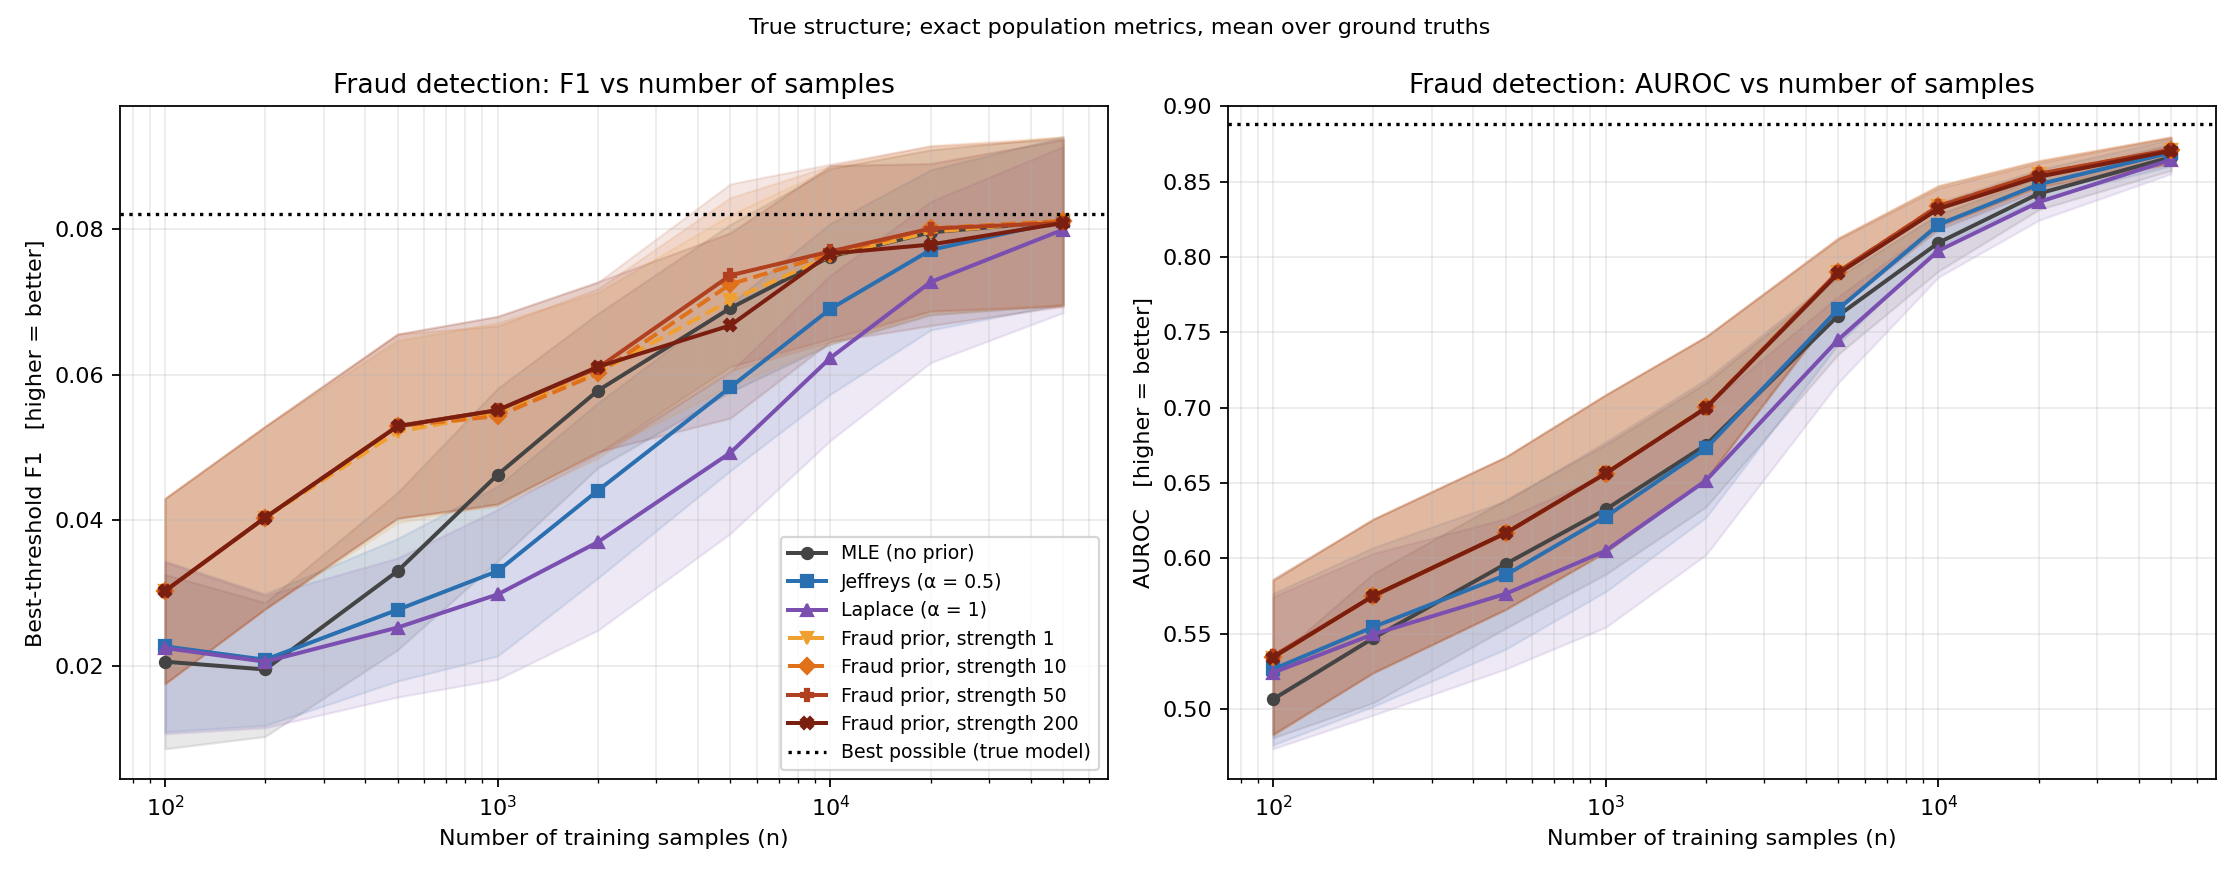
\includegraphics[width=0.78\textwidth]{figs/lc_detection_vs_n.png}
\caption{Fraud detection with the true structure at 0.5\% fraud: (a) oracle-threshold F1 and (b) AUROC against the number of training samples (mean and 95\% confidence interval over 20 worlds). Bands overlap because worlds differ in difficulty; the estimators are compared within each world (see text).}\label{fig:det}
\end{figure*}

\begin{table}[H]
\centering\footnotesize
\begin{adjustbox}{max width=\linewidth}
\begin{tabular}{rcccccccc}\toprule
 & \multicolumn{4}{c}{F1} & \multicolumn{4}{c}{AUROC}\\\cmidrule(lr){2-5}\cmidrule(lr){6-9}
$n$ & MLE & Jeff. & Lap. & FP50 & MLE & Jeff. & Lap. & FP50\\\midrule
100 & 0.021 & 0.023 & 0.023 & 0.030 & 0.506 & 0.526 & 0.524 & 0.535\\
500 & 0.033 & 0.028 & 0.025 & 0.053 & 0.596 & 0.589 & 0.576 & 0.617\\
2,000 & 0.058 & 0.044 & 0.037 & 0.061 & 0.675 & 0.673 & 0.652 & 0.700\\
5,000 & 0.069 & 0.058 & 0.049 & 0.074 & 0.761 & 0.765 & 0.745 & 0.790\\
20,000 & 0.079 & 0.077 & 0.073 & 0.080 & 0.842 & 0.848 & 0.836 & 0.855\\
50,000 & 0.081 & 0.081 & 0.080 & 0.081 & 0.866 & 0.869 & 0.865 & 0.871\\\bottomrule
\end{tabular}
\end{adjustbox}
\caption{Mean oracle-threshold F1 and AUROC (true structure, 0.5\% fraud, 20 worlds; higher is better).}\label{tab:f1}
\end{table}



\subsection{Effect of prior strength and incorrect prior beliefs}
Fig.~\ref{fig:belief} crosses the strength of the fraud prior with the base rate it assumes (true rate 0.5\%). When the assumed rate was correct or too low, strength made almost no difference (AUROC 0.617 at strengths 1 and 500 for $n=500$). When the assumed rate was too high, harm grew with strength: a rate ten times too high cost 0.013 AUROC at strength 10 but 0.045 at strength 50 and 0.075 at strength 200 ($n=5{,}000$). From 2,000 samples, strengths of 50 or more combined with that error were worse than MLE; at 500 samples or fewer even a wrong prior still beat MLE, because MLE is so poor there. A rate only four times too high was safe up to strength 50 at every size. A ``50/50'' belief (100 times too high) at strength 200 cost 0.075 AUROC at 500 samples, 0.243 at 5,000, 0.276 at 20,000 and still 0.258 at 50,000: the damage did not fade as data grew. A strong prior is only safe when the base rate is known well; otherwise a weak prior keeps most of the benefit with little risk.

The fraud-rate experiment points the same way for KL. When the fixed 0.5\% guess is applied at higher true rates (Table~\ref{tab:mis}), the damage grows with strength: at a true rate of 10\% and $n=10{,}000$, KL is 0.073 for $s=10$ and 0.103 for $s=200$, against 0.070 when the prior is centred on the true rate at either strength (Table~\ref{tab:mis}). F1 was almost unaffected by the misspecification at this sample size (0.225 against 0.217 at $s=200$).

\begin{table}[H]
\centering\small
\begin{adjustbox}{max width=\linewidth}\begin{tabular}{rrrrrr}\toprule
Fraud rate & $s$ & KL fixed 0.5\% & KL true rate & F1 fixed 0.5\% & F1 true rate\\\midrule
0.5\% & 10 & 0.0679 & 0.0679 & 0.077 & 0.077\\
 & 50 & 0.0675 & 0.0675 & 0.077 & 0.077\\
 & 200 & 0.0682 & 0.0682 & 0.077 & 0.077\\
\midrule
5\% & 10 & 0.0732 & 0.0697 & 0.154 & 0.154\\
 & 50 & 0.0737 & 0.0688 & 0.153 & 0.154\\
 & 200 & 0.0827 & 0.0703 & 0.150 & 0.153\\
\midrule
10\% & 10 & 0.0732 & 0.0696 & 0.225 & 0.225\\
 & 50 & 0.0785 & 0.0688 & 0.222 & 0.225\\
 & 200 & 0.1031 & 0.0705 & 0.217 & 0.225\\
\bottomrule\end{tabular}\end{adjustbox}
\caption{Fixed (0.5\%) versus true-rate centring of the fraud prior at $n=10{,}000$ (true structure; mean over 20 worlds). $s$ is the prior strength.}\label{tab:mis}
\end{table}

\begin{figure*}[t]
\centering
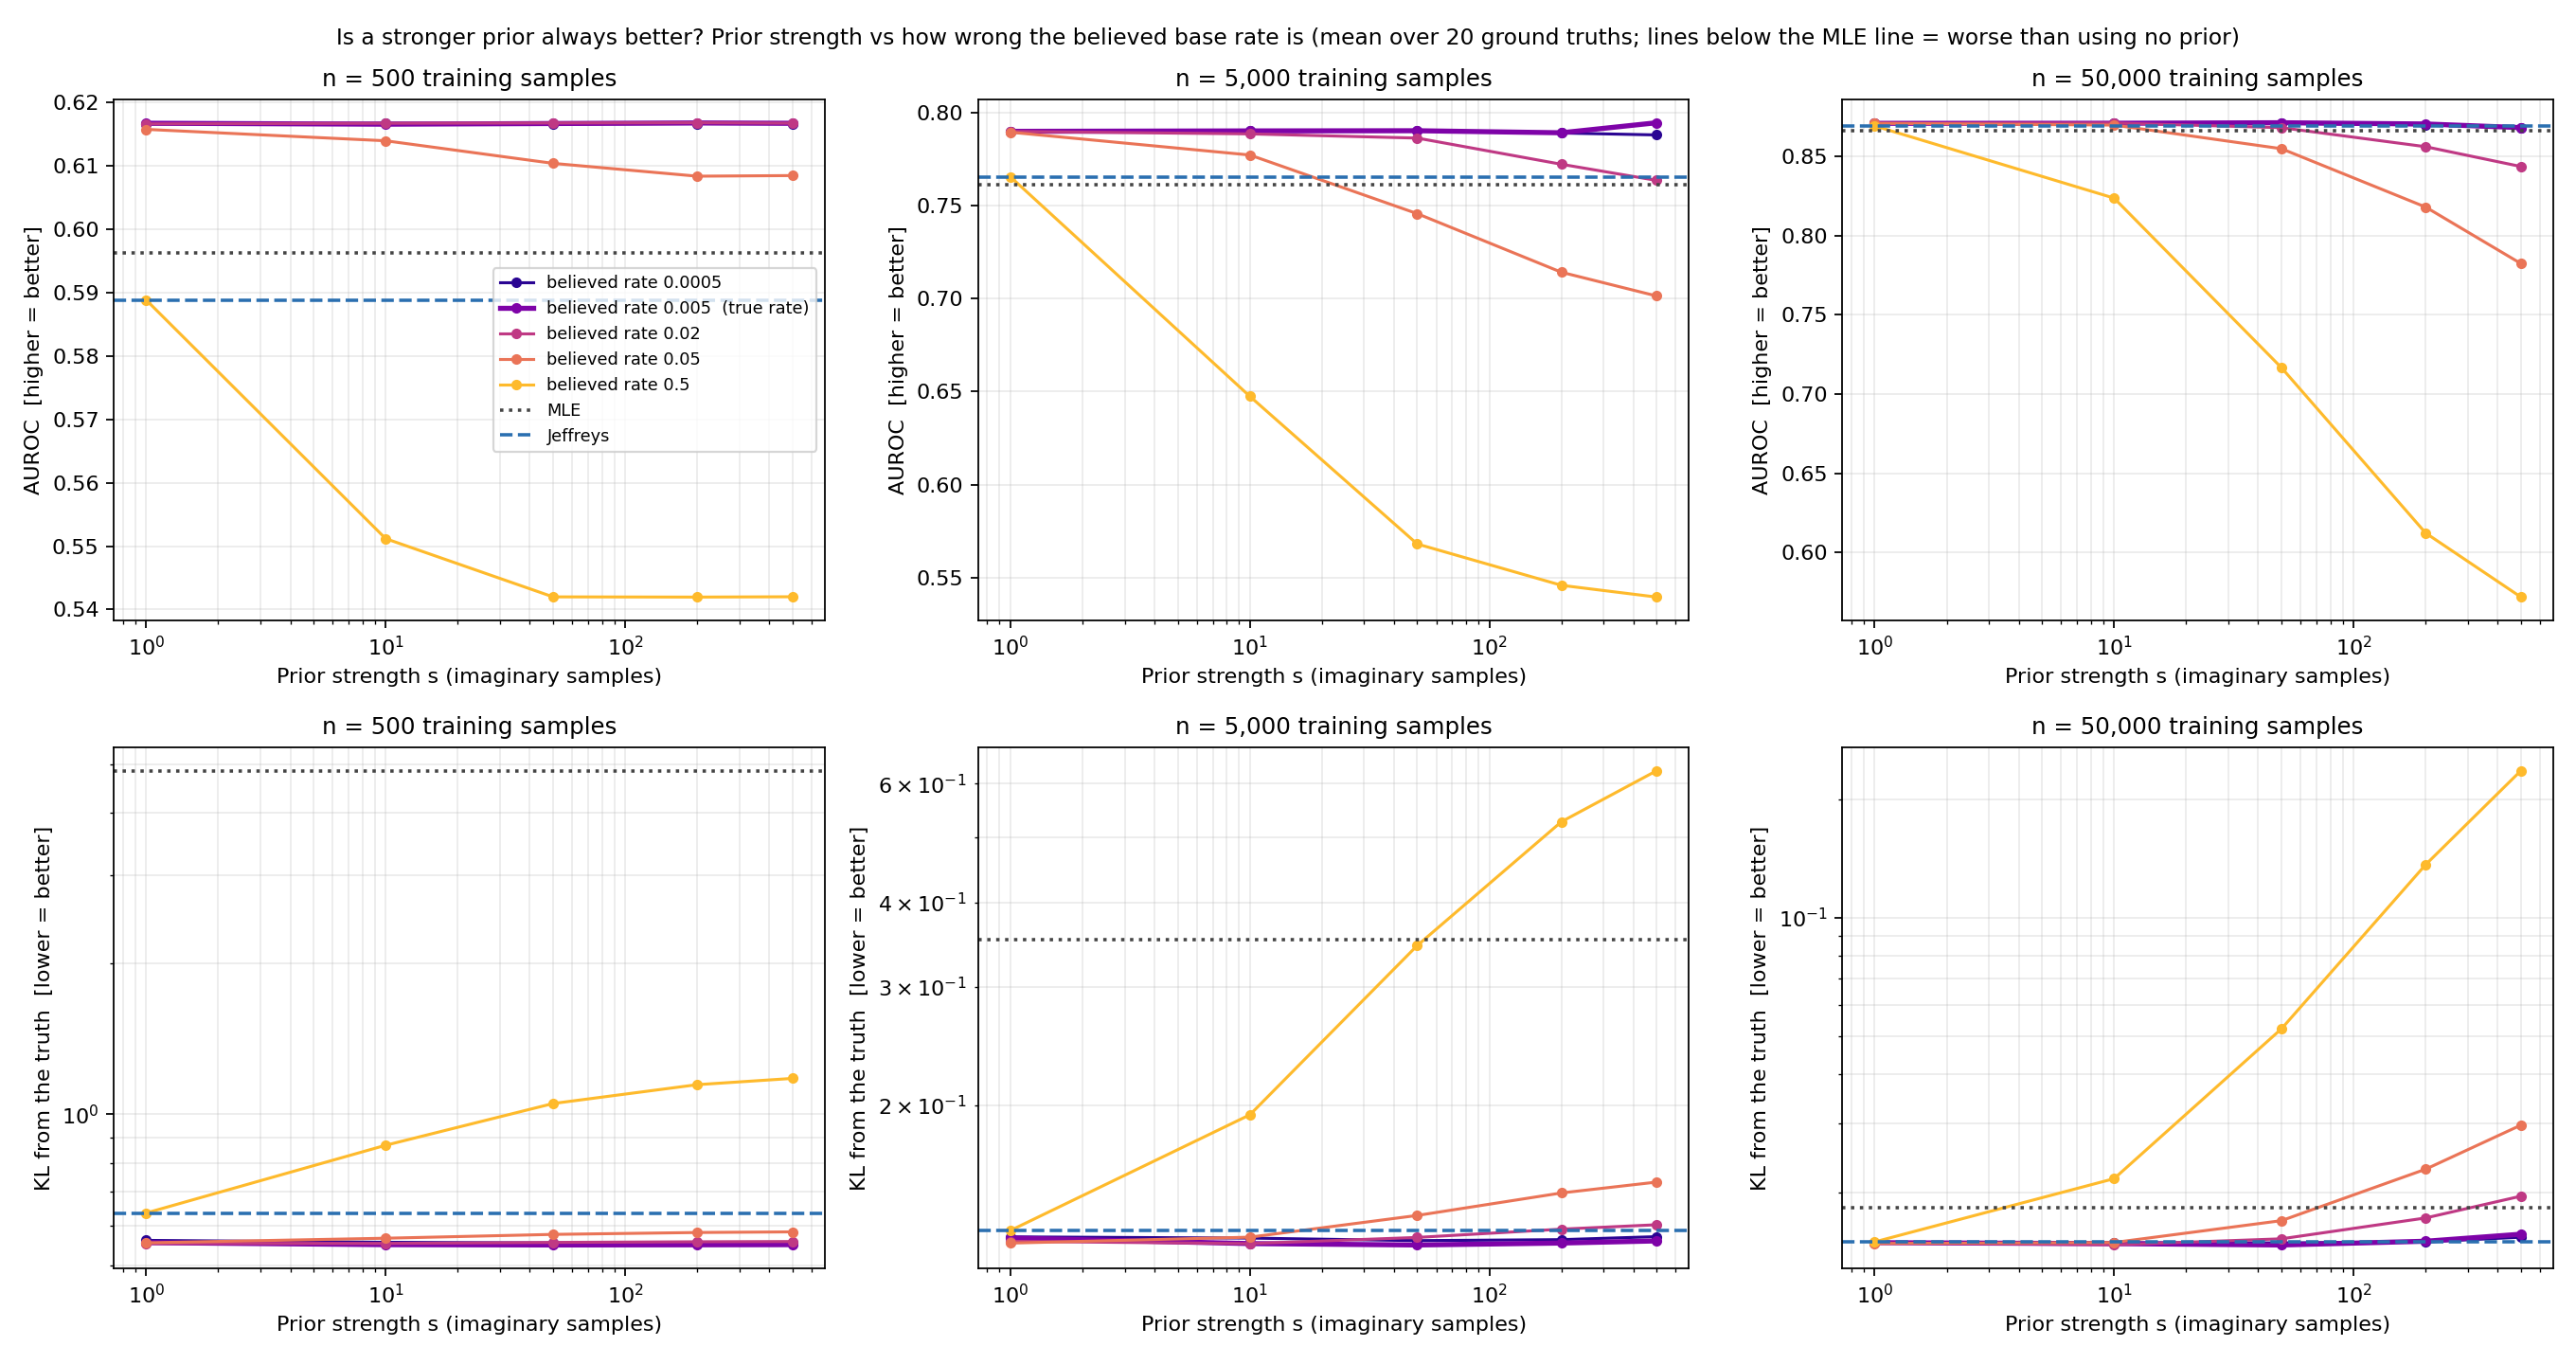
\includegraphics[width=0.42\textwidth]{figs/lc_strength_by_belief.png}
\caption{Prior strength against AUROC (top) and KL divergence (bottom) for five assumed fraud base rates (true rate 0.5\%), at three sample sizes. The dotted line is MLE; curves below it in the top row are worse than using no prior. Mean over 20 worlds.}\label{fig:belief}
\end{figure*}



\subsection{Effect of different true fraud rates}

Fig.~\ref{fig:map} summarizes which estimator is preferable in each condition.

For closeness to the truth, MLE is far from the truth at small $n$ at every fraud rate (KL about 9.5 to 9.9 at 100 rows with the $10^{-4}$ floor, against about 0.85 to 1.15 for the priors). In the corrected map (Fig.~\ref{fig:map}a), the fraud prior was significantly closer than all three standard methods at 100 to 200 rows at fraud rates of 0.1\% and 0.5\%, at 100 rows at 2\%, and at 0.1\% from 20,000 rows. Laplace was significantly closer than the fraud prior from 1,000 rows at 2\% and from 500 rows at 5\% and 10\%. At 0.1\% and 0.5\% fraud between 500 and 10,000 rows no difference was significant. The differences are modest in size (a few to about 20\% in KL between the better priors) compared with the gap to MLE. Laplace also smooths every non-fraud node more strongly than the fraud prior does, so its advantage at higher fraud rates may come from those nodes and not from the fraud node; Section~\ref{sec:fair} tests this by matching the smoothing, and reverses this reading.

For fraud detection, after Holm correction, and requiring the fraud prior to beat MLE as well as Jeffreys and Laplace, it was significantly better in only five of 45 conditions: 500 to 1,000 rows at 0.5\% and 2\% fraud, and 500 rows at 5\% (Fig.~\ref{fig:map}b). It was never significantly better at 0.1\% or 10\% fraud, or from 2,000 rows. The detection benefit of the fraud prior is real but narrow in these worlds, and it is much smaller once MLE is included as a comparator and multiple testing is accounted for.







\begin{figure*}[t]
\centering
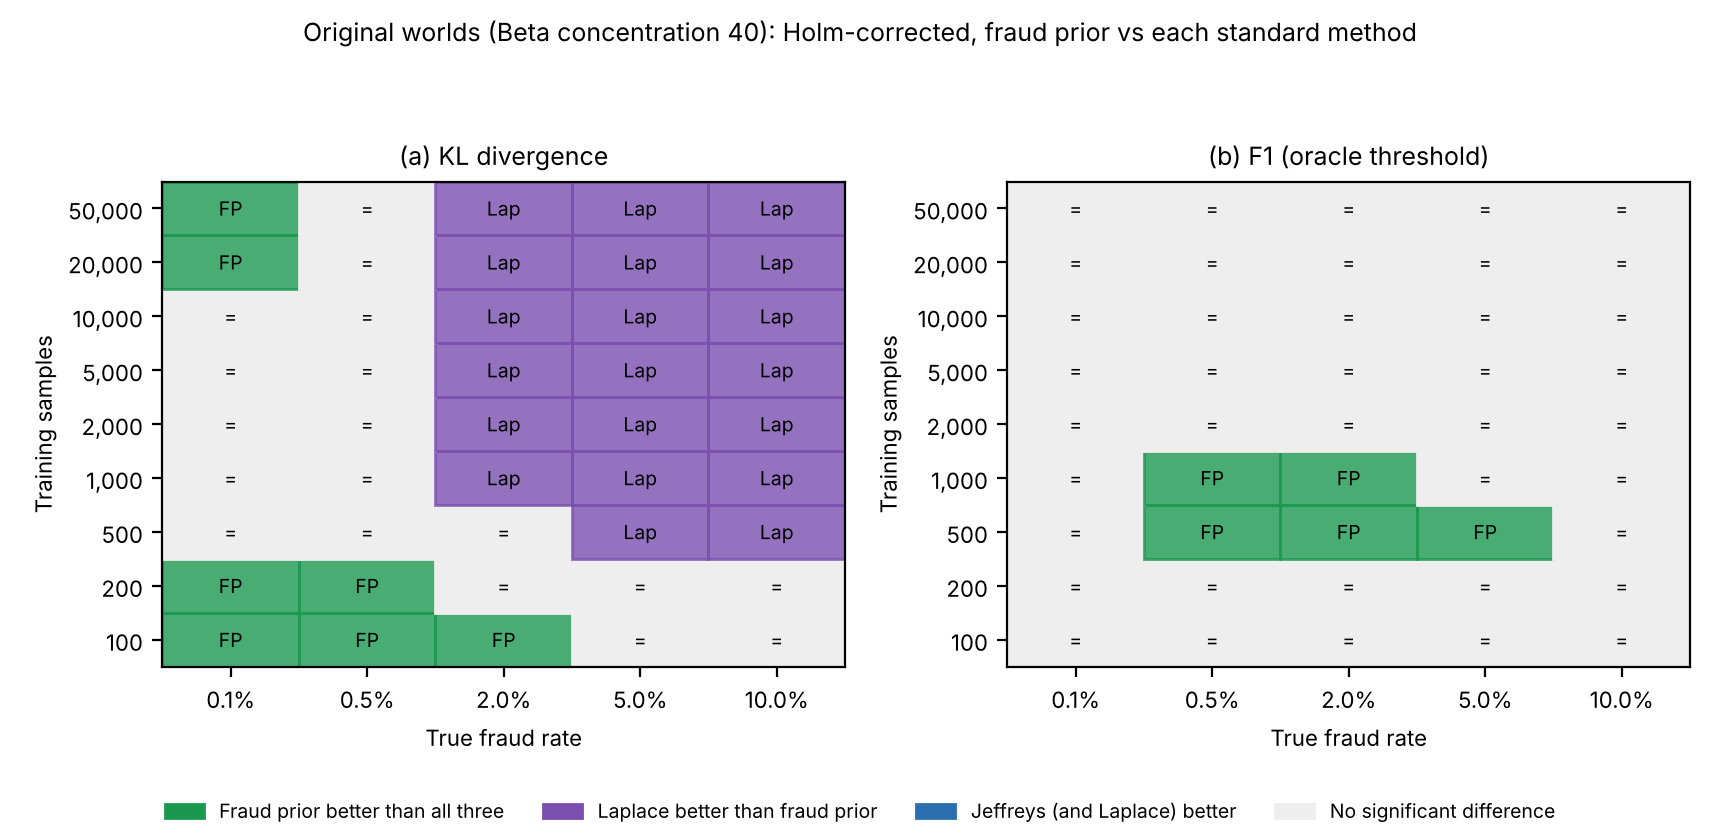
\includegraphics[width=0.5\textwidth]{figs/fr_map.png}
\caption{Holm-corrected map for the original worlds. Each cell compares the fraud prior (strength 50, centred on the true rate) with each of MLE, Jeffreys and Laplace (paired Wilcoxon, 20 worlds, 270 tests corrected together). Green: significantly better than all three; purple or blue: Laplace (or Jeffreys) significantly better than the fraud prior; grey: no significant difference. Exploratory (one prior strength, one generator).}\label{fig:map}
\end{figure*}

\subsection{Controlled predictability}\label{sec:ctrl}
In the controlled worlds the Beta concentration of the fraud probability was solved for each fraud rate (from 579 at 0.1\% to 7.3 at 10\%, against 40 in the original worlds, where best AUROC falls from 0.96 at 0.1\% to 0.64 at 10\%), so the best achievable AUROC is about 0.80 at every fraud rate, so differences between rates are no longer driven by predictability. The KL results were essentially unchanged (Fig.~\ref{fig:mapc}a): the fraud prior was significantly closer at 100 to 200 rows at 0.1\% and 0.5\% and at 100 rows at 2\%, and Laplace (and from 2,000 to 10,000 rows at 5\% to 10\% also Jeffreys) was significantly closer at fraud rates of 2\% and above. For F1 the fraud prior was significantly better than all three standard methods in six of 45 conditions (Fig.~\ref{fig:mapc}b): 1,000 rows at 0.5\%, 500 to 1,000 rows at 2\%, 200 to 500 rows at 5\%, and 200 rows at 10\%. It was never significantly better at 0.1\% fraud, or from 2,000 rows. Holding predictability roughly constant did not remove the small-sample advantage of the fraud prior; it moved it to higher fraud rates (5\% to 10\%), where the original worlds had shown none, and it still vanished by 2,000 rows. The absence of any benefit at 0.1\% fraud, where a 100-row sample holds about 0.1 fraud rows, indicates that a base-rate prior cannot help when samples contain almost no fraud, and part of the original pattern reflected predictability, not prevalence alone.


\begin{figure*}[t]
\centering
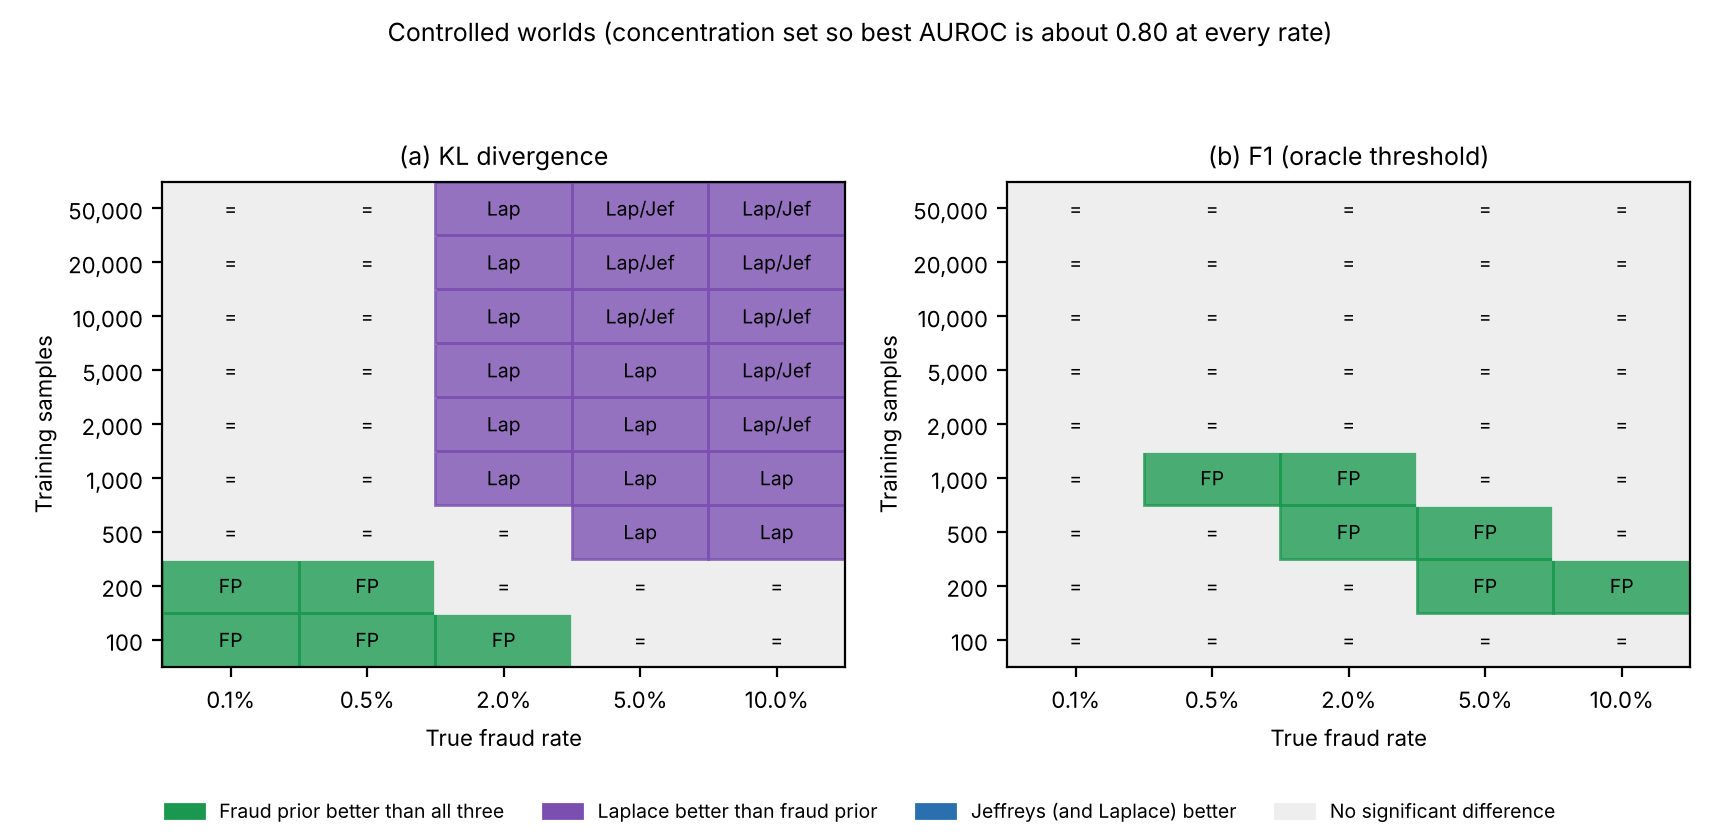
\includegraphics[width=0.5\textwidth]{figs/fr_map_ctrl.png}
\caption{As Fig.~\ref{fig:map}, for the controlled worlds in which the best achievable AUROC is about 0.80 at every fraud rate.}\label{fig:mapc}
\end{figure*}

\subsection{Matched smoothing on the other variables}\label{sec:fair}
The maps above compare the fraud prior with Laplace smoothing, which adds one pseudo-count to every cell of every node, whereas the fraud prior uses a pseudo-count of 0.5 on the non-fraud nodes. A difference between them can therefore come from the other nodes rather than from the fraud node. Table~\ref{tab:fair} compares a fraud prior of strength 50 with Laplace smoothing on every non-fraud node against Laplace smoothing everywhere, so that only the fraud node differs (the existing comparison with Jeffreys smoothing is matched in the same way). With matched smoothing, the fraud prior was closer to the truth in KL in 18 to 20 of 20 worlds at every sample size and at both fraud rates, with the largest gain at 100 rows (about 0.3) and a gain that shrank steadily with $n$. Detection improved as well: the AUROC gain was between 0.01 and 0.05 at 0.5\% fraud up to 10,000 rows and fell to 0.007 at 50,000, and the oracle-threshold F1 gain followed the same pattern (Table~\ref{tab:fair}). The earlier finding that Laplace was closer for KL at fraud rates of 2\% and above is therefore explained by its heavier smoothing of the ordinary variables. The fraud node itself is better estimated by a base-rate prior at every size, and the advantage matters less as fraud rows accumulate.

\begin{table}[H]
\centering\footnotesize
\begin{adjustbox}{max width=\linewidth}\begin{tabular}{rrcccc}\toprule
Fraud rate & $n$ & KL gain (95\% CI) & Closer in & AUROC gain (95\% CI) & F1 gain\\\midrule
0.5\% & 100 & 0.360 (0.299, 0.413) & 20/20 & +0.010 (+0.001, +0.024) & +0.008\\
0.5\% & 500 & 0.137 (0.110, 0.162) & 20/20 & +0.040 (+0.018, +0.067) & +0.028\\
0.5\% & 2,000 & 0.038 (0.029, 0.045) & 19/20 & +0.048 (+0.021, +0.076) & +0.024\\
0.5\% & 10,000 & 0.006 (0.005, 0.008) & 20/20 & +0.030 (+0.020, +0.039) & +0.015\\
0.5\% & 50,000 & 0.001 (0.001, 0.001) & 20/20 & +0.007 (+0.005, +0.009) & +0.001\\
2\% & 100 & 0.316 (0.259, 0.365) & 20/20 & +0.009 (-0.001, +0.020) & +0.006\\
2\% & 500 & 0.112 (0.089, 0.131) & 20/20 & +0.020 (+0.012, +0.029) & +0.023\\
2\% & 2,000 & 0.026 (0.020, 0.031) & 19/20 & +0.028 (+0.020, +0.038) & +0.020\\
2\% & 10,000 & 0.003 (0.002, 0.004) & 19/20 & +0.008 (+0.006, +0.011) & +0.008\\
2\% & 50,000 & 0.000 (0.000, 0.000) & 18/20 & +0.001 (+0.001, +0.002) & +0.000\\
\bottomrule\end{tabular}\end{adjustbox}
\caption{Fraud prior (strength 50, centred on the true rate, Laplace smoothing on all non-fraud nodes) minus Laplace smoothing everywhere, true structure, mean over 20 worlds with 95\% bootstrap intervals over worlds. KL gain: Laplace minus fraud prior (positive means the fraud prior is closer). Closer in: worlds in which the fraud prior had the lower KL. This is an exploratory analysis.}\label{tab:fair}
\end{table}

\subsection{Where the prior's rate comes from}\label{sec:rate}
So far the fraud prior used the generating rate, which no practitioner knows. Table~\ref{tab:rate} gives its AUROC gain over Jeffreys smoothing when the rate was estimated instead from a separate historical sample of 1,000 or 10,000 transactions from the same world, or from the training sample itself, and when it was deliberately ten times too low or too high. The estimated rates gave the same gains as the true rate to within 0.001 at every size, even though individual estimates from 1,000 historical rows ranged from 0.25\% to 1.05\% at a true rate of 0.5\%: with so few fraud rows the prior's effect is to move empty configurations towards a small fraud probability, and the exact value matters little. A rate ten times too low did no harm. A rate ten times too high was harmful from 2,000 rows at 0.5\% fraud and from 500 rows at 2\%, by up to 0.065 AUROC. The historical sample came from the same world, so this assumes no drift.

\begin{table}[H]
\centering\footnotesize
\begin{adjustbox}{max width=\linewidth}\begin{tabular}{rrcccccc}\toprule
Fraud rate & $n$ & True & Hist.\,10k & Hist.\,1k & Training & $0.1\times$ & $10\times$\\\midrule
0.5\% & 100 & +0.008 & +0.009 & +0.009 & +0.008 & +0.007 & +0.007\\
0.5\% & 500 & +0.028 & +0.028 & +0.028 & +0.028 & +0.028 & +0.018\\
0.5\% & 2,000 & +0.027 & +0.027 & +0.027 & +0.027 & +0.027 & -0.001\\
0.5\% & 10,000 & +0.012 & +0.012 & +0.012 & +0.012 & +0.012 & -0.026\\
0.5\% & 50,000 & +0.002 & +0.002 & +0.002 & +0.002 & +0.002 & -0.014\\
2\% & 100 & +0.006 & +0.007 & +0.007 & +0.007 & +0.006 & -0.003\\
2\% & 500 & +0.011 & +0.011 & +0.011 & +0.011 & +0.011 & -0.014\\
2\% & 2,000 & +0.014 & +0.014 & +0.014 & +0.014 & +0.013 & -0.060\\
2\% & 10,000 & +0.003 & +0.003 & +0.003 & +0.003 & -0.000 & -0.065\\
2\% & 50,000 & +0.000 & +0.000 & +0.000 & +0.000 & -0.001 & -0.027\\
\bottomrule\end{tabular}\end{adjustbox}
\caption{AUROC gain of the fraud prior (strength 50, Jeffreys smoothing elsewhere) over Jeffreys smoothing, by where the prior's rate comes from (true structure, mean over 20 worlds). True: generating rate; Hist.: rate estimated from a separate sample of 1,000 or 10,000 rows; Training: rate estimated from the training sample; $0.1\times$ and $10\times$: the true rate multiplied by 0.1 or 10.}\label{tab:rate}
\end{table}

\subsection{Why Hill Climbing misses fraud: a direct test}\label{sec:mech}
The edge-recovery results show that fraud edges are rarely learned, but not why. Hill Climbing adds an edge only if the BIC score rises, that is, if the log-likelihood gain exceeds a penalty of $\tfrac12\ln n$ per extra parameter. Table~\ref{tab:mech} and Fig.~\ref{fig:mech}a give the average gain and penalty for adding a single true parent to a fraud node with no parents. At 100 rows (0.7 fraud rows on average) the gain was 0.9 against a penalty of 9.2. The gain grew roughly in proportion to the number of fraud rows, whereas the penalty grew only with $\ln n$, so the net change in BIC rose from $-8$ at 100 rows to $-4$ at 20,000 rows and was positive ($+13.5$) only at 50,000 rows, where 59\% of the true fraud edges paid for themselves. Adding all true parents at once never paid in more than 20\% of worlds at any size. These averages include weak edges; the proportion of edges that pay is the quantity that matters, and it rose from 2\% at 5,000 rows to 17\% at 20,000 and 59\% at 50,000. The share of worlds in which Hill Climbing actually linked the fraud node followed the same course (5\%, 45\% and 85\% at 2,000, 20,000 and 50,000 rows), and is higher than the share of single edges that pay because a world needs only one edge to be linked. We then followed the actual search (Table~\ref{tab:mech}). Hill Climbing accepted about 14 moves per world at 50,000 rows, nearly all between ordinary variables. Up to 5,000 rows, when it stopped in a world without a fraud edge, the best remaining move involving the fraud node would still have lowered BIC by 8 to 10 (median), which matches the single-edge deficit of 8 to 12 and shows that the single-edge test describes the decisions the search faced after other edges had been added. When a fraud edge was accepted it came late, after a median of 8 to 12 other accepted moves from 10,000 rows, and fraud moves were 1\% to 9\% of all accepted moves. At 20,000 rows the deficit shrank to about 3. We validated our search against pgmpy's Hill Climbing on the same 180 runs. They agreed on whether the fraud node was linked in every run. Up to 1,000 rows the learned graphs were Markov equivalent (same skeleton and v-structures, hence the same BIC) in every run, and over all sizes in 68\% of runs; the remainder were at larger samples, where the two greedy searches stopped at different local optima, ours with the higher BIC in 20\% of runs and pgmpy's in 12\%. The fitted models differed little (mean absolute AUROC difference 0.0015, at most 0.048), and their mean curves were almost identical: at every sample size the average AUROC differed by at most 0.003, the average KL by at most 0.02, and the share of runs linking the fraud node was the same (30\%, 45\% and 85\% at 10,000, 20,000 and 50,000 rows). The penalty need not be the only cause of missing fraud edges, since search order, competing edges and local optima also matter.

The same table shows how the improvement unfolds. Distribution approximation improved gradually, because most of the 14 learned edges join ordinary variables, all of which have plenty of informative rows: the learned graph already had nine edges at 10,000 rows, and its KL fell from 0.72 at 500 rows to 0.38 at 10,000 and 0.04 at 20,000. Detection did not improve gradually. In worlds where no fraud edge had been learned, AUROC stayed at 0.50 at every sample size, and in worlds where one had been learned it was between 0.73 and 0.87. The mean AUROC (0.52, 0.58, 0.60, 0.70 at 5,000, 10,000, 20,000 and 50,000 rows) therefore rises only because more worlds acquire a fraud edge, and the transition around 20,000 rows is where the likelihood gain from fraud edges starts to approach the penalty.

\begin{table}[H]
\centering\footnotesize
\begin{adjustbox}{max width=\linewidth}\begin{tabular}{rrrrrrrrrr}\toprule
$n$ & Fraud rows & $\Delta$LL & Penalty & $\Delta$BIC & Edges paying & Search stop $\Delta$BIC & Worlds linked & First fraud step & AUROC\\\midrule
100 & 0.7 & 0.9 & 9.2 & -8.3 & 0\% & -7.6 & 0\% & -- & 0.50\\
200 & 1.4 & 1.3 & 10.6 & -9.3 & 0\% & -8.8 & 0\% & -- & 0.50\\
500 & 3.1 & 2.4 & 12.4 & -10.0 & 0\% & -8.7 & 0\% & -- & 0.50\\
1,000 & 5.7 & 2.7 & 13.8 & -11.1 & 0\% & -9.3 & 0\% & -- & 0.50\\
2,000 & 11.4 & 3.6 & 15.2 & -11.6 & 2\% & -10.1 & 5\% & 3 & 0.52\\
5,000 & 26.5 & 5.9 & 17.0 & -11.1 & 2\% & -9.9 & 5\% & 5 & 0.52\\
10,000 & 54.0 & 9.2 & 18.4 & -9.3 & 11\% & -9.6 & 30\% & 8 & 0.58\\
20,000 & 106.7 & 15.9 & 19.8 & -3.9 & 17\% & -3.1 & 45\% & 11 & 0.60\\
50,000 & 258.5 & 35.2 & 21.6 & +13.5 & 59\% & -4.1 & 85\% & 12 & 0.70\\
\bottomrule\end{tabular}\end{adjustbox}
\caption{Adding one true parent to the fraud node (0.5\% fraud, 20 worlds, 54 true fraud edges). $\Delta$LL and Penalty: mean log-likelihood gain and BIC penalty; $\Delta$BIC: their difference; Edges paying: share of true edges with $\Delta$BIC $>0$. Search stop $\Delta$BIC: median $\Delta$BIC of the best remaining move involving the fraud node when the traced search stopped in a world with no fraud edge. Worlds linked and first fraud step (number of accepted moves before it, median): traced search. AUROC: Hill Climbing run of the learning curves (Laplace parameters), mean over worlds.}\label{tab:mech}
\end{table}

\begin{figure*}[t]
\centering
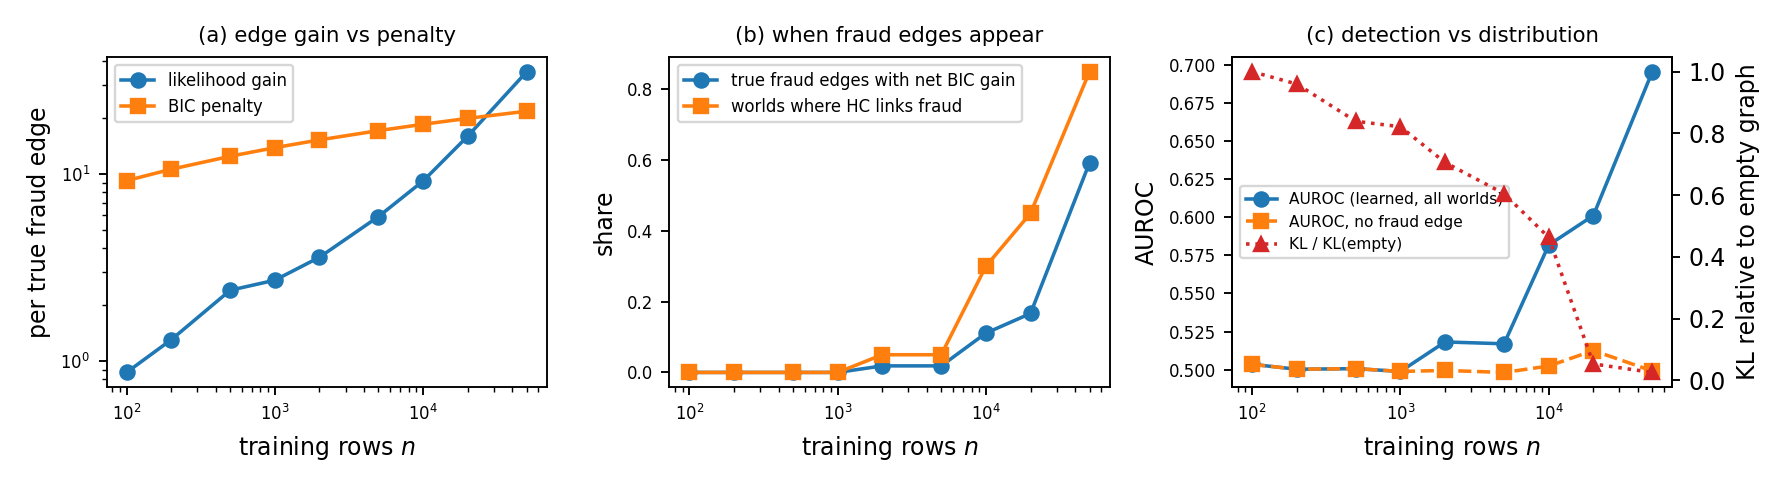
\includegraphics[width=0.72\textwidth]{figs/mechanism.png}
\caption{(a) Mean log-likelihood gain and BIC penalty of adding a true fraud edge. (b) Share of true fraud edges that pay for themselves and share of worlds in which Hill Climbing linked the fraud node. (c) AUROC of the learned network (all worlds, and worlds with no fraud edge) and KL relative to the empty graph. Twenty worlds, 0.5\% fraud.}\label{fig:mech}
\end{figure*}

\subsection{Learned structures: the fraud prior and structure learning compete}\label{sec:learned}
With the Hill Climbing structure the priors still gave a lower KL than MLE in nearly every world, but the gain was small next to structural error: up to 10,000 samples all estimators had nearly the same KL, and detection was identical across them (median AUROC 0.50 until 20,000 rows, which is chance). The reason is visible in the graph. At 50,000 rows the true fraud node had on average 2.7 parents (about 103 parent configurations), whereas the learned fraud node had about 1.4 parents (about 13 configurations) when it had any. A prior helps by filling empty configurations, and a node with few configurations has few empty ones.

Table~\ref{tab:struct} compares structures that are learned rather than given, with the fraud prior measured against Jeffreys smoothing so that only the fraud node differs. In the original worlds, Hill Climbing connected the fraud node to a variable in 30\% of runs, and the fraud prior was indistinguishable from smoothing (mean AUROC difference below 0.001). Naive Bayes and TAN gave fraud a single parent configuration, so the prior reduced to a base-rate estimate and made no difference (below 0.001). The latent-class generator showed the same division. With the fixed three-parent structure, the fraud prior improved AUROC over Jeffreys smoothing by 0.015 (better in 59\% of 500 runs). With Hill Climbing the difference was $+0.001$ and with naive Bayes it was zero. The last column of the table explains why: the share of runs in which the fraud node both had parents and had fewer than three expected fraud rows per configuration was 0.80 for the fixed structure and 0.01 for Hill Climbing. Structure learning gave the fraud node either no parents or few, well-populated configurations, so it removed the shortage of fraud cases that the prior is meant to address. The two remedies are largely alternatives: a prior can matter only for a structure that gives fraud many parents, and Hill Climbing with BIC does not learn such a structure when fraud is rare.

\begin{table}[H]
\centering\footnotesize
\begin{adjustbox}{max width=\linewidth}\begin{tabular}{llrcccccc}\toprule
World & Structure & $q$ & Parents & Niche & MLE & Jeff. & FP50 & FP50$-$Jeff.\\\midrule
Original & HC & 5 & 0.4 & 0.01 & 0.565 & 0.566 & 0.566 & -0.0005\\
Original & NB & 1 & 0.0 & 0.00 & 0.604 & 0.607 & 0.607 & -0.0000\\
Original & TAN & 1 & 0.0 & 0.00 & 0.608 & 0.617 & 0.617 & -0.0000\\
Latent & FParents & 125 & 3.0 & 0.80 & 0.680 & 0.688 & 0.703 & +0.0151\\
Latent & HC & 7 & 0.6 & 0.01 & 0.617 & 0.615 & 0.616 & +0.0008\\
Latent & NB & 1 & 0.0 & 0.00 & 0.688 & 0.698 & 0.698 & -0.0000\\
\bottomrule\end{tabular}\end{adjustbox}
\caption{Learned structures with and without the fraud prior (mean AUROC over all runs). $q$: mean number of parent configurations of the fraud node; Parents: mean number of fraud parents; Niche: share of runs in which the fraud node had parents and $k<3$. Original worlds: 20 worlds, fraud rates 0.5\% and 2\%, four sizes (160 runs per row). Latent-class generator: 20 worlds, five rates, five sizes (500 runs per row). FParents: fixed three-parent structure. Jeff.: Jeffreys smoothing on every node. Differences are uncorrected for multiple testing.}\label{tab:struct}
\end{table}

\subsection{Real fraud data}\label{sec:real}
Table~\ref{tab:real} gives held-out AUROC on the credit-card data. Hill Climbing left the fraud node unconnected at 1,000 and 5,000 rows (AUROC about 0.5, with two to eight fraud rows) and became useful only at 20,000 rows, as in the synthetic worlds. Naive Bayes and TAN reached AUROC of 0.89 to 0.97 from the same two to eight fraud rows. Smoothing mattered: with two fraud rows, MLE ranked transactions far worse than smoothed estimators for naive Bayes and TAN (AUROC lower by about 0.09 and 0.075; $p<0.001$ after Holm correction), because MLE gives probability zero to every unseen combination, and the gap closed as fraud rows accumulated. The fraud prior added nothing beyond smoothing with these structures: its AUROC was identical to Jeffreys smoothing to three decimals at every size. For Hill Climbing the fraud prior was higher than Jeffreys smoothing by 0.02 at 1,000 rows and 0.03 at 5,000, but with 30 repeats this was not significant (uncorrected $p=0.87$ and $0.32$) and the unconnected graphs were close to chance in both cases. To see why naive Bayes and TAN outperform Hill Climbing here, we traced the search on the real data (30 repeats). Hill Climbing linked the fraud node in none of the repeats at 1,000 rows (two fraud rows), in 13\% at 5,000 rows (eight fraud rows) and in all of them at 20,000 rows (34 fraud rows). When it linked fraud it connected one or two of the eight features, nearly always the one or two most informative about the label (on average 2.0 features at 60,000 rows). In the unlinked repeats the best remaining fraud move would still have lowered BIC by 10.5 (1,000 rows) and 5.6 (5,000 rows) in the median, so no single feature passed the penalty, although together the features carry much more information: naive Bayes, which connects all eight, reached AUROC 0.89 at 1,000 rows and 0.97 at 5,000. A score that tests one edge at a time cannot add up many weak pieces of evidence, whereas a structure with the fraud node at the root adds them by construction. From 20,000 rows Hill Climbing caught up (AUROC 0.86 to 0.95) as the strongest features passed the penalty, but it still used fewer features than naive Bayes, which was at 0.97 at 20,000 rows. This is a comparison of modelling strategies and not of structure-learning algorithms under identical constraints: naive Bayes and TAN impose the connections to the fraud label, whereas Hill Climbing must discover them. Imposing a structure adds bias, because the features need not all depend on fraud in that way, but removes the variance of deciding each edge from a handful of fraud rows; with so few fraud rows the reduction in variance outweighed the bias, and the gap in AUROC narrowed from about 0.4 at 1,000 rows to about 0.03 with the whole training set. The fraud prior was not better than Laplace smoothing either. This is consistent with the guidelines of Section~\ref{sec:guide} and does not contradict them: with a class-rooted structure there is one parent configuration with two or more fraud rows, so $k$ is above the range in which a prior matters, and with Hill Climbing the fraud node has no parents. The real data contain no structure in which the fraud node has many parents and few fraud rows, so they cannot test the rule, only show that it is not needed with these structures.

\begin{table}[H]
\centering\footnotesize
\begin{adjustbox}{max width=\linewidth}\begin{tabular}{rrcccccccccc}\toprule
 & & \multicolumn{3}{c}{Hill Climbing} & \multicolumn{3}{c}{Naive Bayes} & \multicolumn{3}{c}{TAN}\\\cmidrule(lr){3-5}\cmidrule(lr){6-8}\cmidrule(lr){9-11}
$n$ & Fraud rows & MLE & Jeff. & FP50 & MLE & Jeff. & FP50 & MLE & Jeff. & FP50\\\midrule
1,000 & 2 & 0.471 & 0.423 & 0.446 & 0.798 & 0.891 & 0.891 & 0.838 & 0.913 & 0.913\\
5,000 & 8 & 0.479 & 0.544 & 0.575 & 0.920 & 0.969 & 0.969 & 0.897 & 0.940 & 0.940\\
20,000 & 34 & 0.861 & 0.858 & 0.867 & 0.947 & 0.970 & 0.970 & 0.928 & 0.939 & 0.939\\
60,000 & 104 & 0.933 & 0.932 & 0.930 & 0.962 & 0.972 & 0.972 & 0.945 & 0.950 & 0.950\\
\bottomrule\end{tabular}\end{adjustbox}
\caption{Held-out AUROC on the credit-card fraud data (mean over 30 repeats). Fraud rows: mean number of fraud rows in the training sample. FP50: fraud prior of strength 50 centred on the training fraud rate. Jeff.: Jeffreys smoothing on every node.}\label{tab:real}
\end{table}

\subsection{When to prefer a fraud-informed prior}\label{sec:guide}
Table~\ref{tab:guide} gives the AUROC gain of the fraud prior (strength 50, centred on the true rate) over Jeffreys smoothing, which treats every other node identically, grouped by $k$, for three generators with the fraud node's parents fixed. In the original and controlled worlds the average gain was +0.016 and +0.013 when $k<0.3$, +0.009 and +0.011 for $k$ between 0.3 and 1, +0.003 and +0.002 between one and three, and about zero above three. The latent-class generator, whose joint distribution has no sparse network, gave the same shape (+0.027, +0.011, +0.002 and then $-0.001$). The gains are modest. Plotted against the number of rows or the fraud rate separately, the gains differed between worlds; against $k$ they followed a similar curve in all three generators. The gain was positive in 63\% to 92\% of runs when $k<3$ and in 12\% to 61\% of runs when $k>10$, so the prior did not help in every run. Because parent configurations are not equally frequent, we also computed measures from the actual fraud counts per configuration of the fraud node (Table~\ref{tab:kmeas}). The gain in KL was predicted about as well by $k$ (cross-validated $R^2=0.62$) as by the share of configurations with no fraud row (0.65) or a mass-weighted count (0.63), and better than total fraud rows (0.54) or the median count per configuration (0.09, since the median is zero in nearly all runs). The gain in AUROC was much less predictable: every measure explained only 6\% to 14\% of its variance, with the per-configuration measures (0.13 to 0.14) slightly ahead of total fraud rows (0.06). Counting fraud by configuration is therefore more informative than counting it overall, but the more detailed measures do not improve materially on $k$, and the guideline describes the average gain and not the gain in a single run. Prior strength and belief matter next (Table~\ref{tab:strength}). When the prior placed no more pseudo-fraud rows in each configuration than the data supplied ($\varphi\le1$), the average gain was positive at every believed rate, even one ten or more times the truth ($+0.006$). Harm appeared only when $\varphi>1$ and the believed rate was ten or more times too high ($-0.008$ for $\varphi$ between one and three, $-0.032$ and $-0.081$ above three); a believed rate ten times too low was not harmful at any strength.

\begin{table}[H]
\centering\footnotesize
\begin{adjustbox}{max width=\linewidth}\begin{tabular}{lccccc}\toprule
World & $k=$ $<0.3$ & $k=$ 0.3--1 & $k=$ 1--3 & $k=$ 3--10 & $k=$ $>10$\\\midrule
Original & +0.016 (+0.012, +0.021) & +0.009 (+0.007, +0.011) & +0.003 (+0.002, +0.004) & +0.001 (+0.001, +0.001) & +0.000 (+0.000, +0.000)\\
Controlled & +0.013 (+0.011, +0.015) & +0.011 (+0.009, +0.013) & +0.002 (+0.001, +0.002) & -0.001 (-0.002, +0.000) & -0.000 (-0.001, -0.000)\\
Latent-class & +0.027 (+0.015, +0.039) & +0.011 (+0.005, +0.016) & +0.002 (-0.000, +0.004) & -0.001 (-0.003, -0.000) & -0.001 (-0.002, -0.001)\\
\bottomrule\end{tabular}\end{adjustbox}
\caption{Mean AUROC gain of the fraud prior (strength 50, true-rate centre) over Jeffreys smoothing, by expected fraud rows per configuration $k$ (true parents fixed), with 95\% bootstrap intervals over worlds in brackets. Original and controlled: 20 worlds, five rates, nine sizes; latent-class: 20 worlds, five rates, five sizes.}\label{tab:guide}
\end{table}

\begin{table}[H]
\centering\footnotesize
\begin{adjustbox}{max width=\linewidth}\begin{tabular}{lcc}\toprule
Measure & KL gain & AUROC gain\\\midrule
Total fraud rows & 0.54 & 0.06\\
$k=n\pi/q$ (mean per configuration) & 0.62 & 0.12\\
Median fraud rows per configuration & 0.09 & 0.06\\
Share of configurations with no fraud row & 0.65 & 0.14\\
Probability mass of those configurations & 0.61 & 0.13\\
Mass-weighted fraud rows (capped at 10) & 0.63 & 0.14\\
\bottomrule\end{tabular}\end{adjustbox}
\caption{Cross-validated $R^2$ of a binned fit of the fraud prior's gain over Jeffreys smoothing on each measure of fraud counts (360 runs: 20 worlds, two fraud rates, nine sizes; true structure).}\label{tab:kmeas}
\end{table}

\begin{table}[H]
\centering\footnotesize
\begin{adjustbox}{max width=\linewidth}\begin{tabular}{lcccc}\toprule
$\varphi=sr_b/k$ & $0.1\times$ & $1\times$ & $4\times$ & $\ge10\times$\\\midrule
$\le1$ & +0.013 & +0.012 & +0.011 & +0.006\\
1--3 & +0.024 & +0.017 & +0.010 & -0.008\\
3--10 & +0.021 & +0.019 & +0.001 & -0.032\\
>10 & +0.017 & +0.022 & +0.013 & -0.081\\
\bottomrule\end{tabular}\end{adjustbox}
\caption{Mean AUROC gain over Jeffreys smoothing by relative prior strength $\varphi=s\,r_b/k$ (rows) and believed rate relative to the true rate (columns), original worlds at 0.5\% fraud, true structure ($s$ from 1 to 500; 20 worlds, six sizes). The $\ge10\times$ column pools ratios of 10 and 100.}\label{tab:strength}
\end{table}

These results suggest the following exploratory guidelines. They describe what held on average in the tested synthetic worlds with the fraud node's parents fixed. They indicate when a benefit may occur and do not guarantee one, they are not established rules, and the thresholds were read from binned averages without validation on real data.
\begin{enumerate}
\item Compute $k=n\pi/q$ for the fraud node of the structure in use. When $k>3$ the average gain of a fraud prior over ordinary smoothing was negligible (below 0.005 AUROC), so the choice among smoothed estimators mattered little.
\item When $k<3$ and the fraud node has parents, a fraud prior centred on a reasonable base rate gave the largest average gain in the tested settings, although it did not help in every run. A rate estimated from a separate sample of 1,000 rows, or from the training sample, did as well as the true rate (assuming no drift), so knowing the exact rate is not required, but a large overestimate is harmful (Table~\ref{tab:rate}).
\item Keep the prior no stronger than the data it replaces, $s\le n/q$, which keeps $\varphi$ near or below one when the believed rate is near the true one. In the tests this setting was never harmful on average, even for a believed rate ten or more times too high.
\item MLE gave a lower AUROC and a far larger KL than smoothed estimators on average whenever $k<10$ in the synthetic worlds, and was much worse on the real data, so some smoothing is advisable. If the structure leaves the fraud node with no parents ($q=1$), the prior reduces to a base-rate estimate and ordinary smoothing was enough.
\item Imbalance enters only through the fraud rate $\pi$ in $k$: for a fixed sample size a rarer class gives a smaller $k$, so the range of sample sizes in which the prior may matter extends in proportion to $1/\pi$.
\end{enumerate}

\subsection{Comparison with models from other paradigms}\label{sec:bench}
The models here were not tuned, so this is a descriptive comparison and not a definitive ranking of model families. On the same 20 worlds and training samples (0.5\% fraud) we trained logistic regression, a linear support vector machine, a decision tree, a random forest \citep{breiman2001}, a one-hidden-layer neural network and naive Bayes \citep{friedman1997}, without class weights or resampling; scores for all $5^8$ feature combinations were weighted by the true probabilities, so AUROC and F1 are exact. With the true structure and the fraud prior the Bayesian network was significantly better than every other model at every size from 500 to 50,000 rows (paired Wilcoxon, $p\le0.005$), which is an upper reference, not a fair contest, because it has the generating model class and the true graph. With the structure learned by Hill Climbing the picture reversed: at 20,000 rows the learned network had lower AUROC and F1 than every other model, and at 50,000 rows its AUROC (0.695) matched logistic regression, the linear SVM and naive Bayes but was below the random forest (0.738) and the neural network (0.785). These comparisons are uncorrected for multiple testing.

\subsection{Why structure learning struggles under imbalance}
The distribution learned by Hill Climbing with BIC was close to the ground truth in KL divergence only with large samples, and until then the fraud node was usually left unconnected, so the model could not detect fraud at all (RQ1). Section~\ref{sec:mech} gives evidence for the mechanism. The likelihood gain from linking the fraud variable to another variable is limited by the information in the fraud rows, so it grows with their number, while the BIC penalty grows only with the number of extra parameters and $\ln n$. For a rare class the gain therefore stays below the penalty until enough fraud rows have been seen, and the learned graph improves gradually for ordinary variables but only suddenly, world by world, for fraud. The real-data runs and the naive Bayes and TAN results show the practical remedy: fixing the fraud node at the root of the graph removes the search problem, and these structures detected fraud from two to eight training fraud rows. This agrees with the argument of \citet{friedman1997} that a likelihood-based score does not focus on the class variable and that naive Bayes can compete with learned general networks for classification.

\subsection{Why priors help when data are scarce, and why Laplace looked best for KL}
Any prior recovered the distribution far faster than MLE (RQ2), as expected of regularization when most parent configurations are sparse: with few rows MLE assigns zero to most unseen cells and pays heavily in KL, which is why its KL at 100 rows is about 9.5 at every fraud rate. For detection the fraud prior performed best when each configuration held very few fraud rows. A plausible reason is that a symmetric prior gives a configuration that is rare or unseen a fraud probability near one half, inflating its score, whereas the fraud prior gives it about the base rate; the dependence on $k$ is consistent with this, since $k$ measures how often a configuration is unseen. Laplace looked closest in KL at fraud rates of 2\% and above only because it smooths the many ordinary variables more heavily (Section~\ref{sec:fair}). KL is dominated by those variables, whereas detection depends only on how the rare class is ranked across the configurations of the fraud node, which is why the best estimator for KL need not be the best for detection. The sensitivity of rare-class probabilities to the assumed class prior parallels the effects documented for undersampling and cost-sensitive decisions \citep{dalpozzolo2015,elkan2001}.

\subsection{Relation to earlier work}
The results agree with earlier work in several respects and add to it in others. The sensitivity of a learned structure to a prior-strength parameter was shown for BDeu scores by \citet{silander2007}; our BIC-based search has no such parameter, and the direct test of Section~\ref{sec:mech} shows a different obstacle, a score that cannot pay for a fraud edge until many fraud rows are seen. The competitiveness of naive Bayes with learned networks for classification \citep{friedman1997} is reproduced here on fraud data, where it is more pronounced because the class is rare. The effect of the assumed class prior on rare-class probabilities has been studied for undersampling \citep{dalpozzolo2015} and cost-sensitive decisions \citep{elkan2001}, but there the prior is changed after the model is fitted. Here it is part of the fitting, and the gain is confined to configurations with few fraud rows. The earlier Bayesian-network studies of fraud \citep{ezawa1995,maes2002,kirkos2007} report predictive scores on real data, which cannot show how far a learned model is from the truth, the question that the exact evaluation here addresses.

\section{Conclusions, Limitations and Future Work}
\subsection{Conclusions}
A Bayesian network learned with Hill Climbing and BIC approximated the ground-truth distribution closely only with large samples (about 20,000 rows at 0.5\% fraud); before that it was barely better than a model with no edges and usually left the fraud node unconnected. A direct test, supported by tracing the search itself, provided evidence that the likelihood gain from a true fraud edge stays below the BIC penalty until roughly 20,000 to 50,000 rows, and that detection improves world by world as fraud edges appear, while distribution approximation improves gradually through the ordinary variables. The same happened on real card data, where Hill Climbing reached useful AUROC only from 20,000 rows.

With the true structure, every prior beat MLE for KL when data were scarce. When the smoothing of all other variables was held identical, a fraud-rate prior was closer to the truth in KL and better in detection than ordinary smoothing at every size tested, with gains that shrank as fraud rows accumulated; the earlier advantage of Laplace in KL at higher fraud rates came from its heavier smoothing of the other variables. After correction for multiple comparisons against all three standard estimators, including MLE, the fraud prior gave significantly better oracle-threshold F1 only for a few hundred to about 1,000 rows, and a strong prior centred on a rate ten or more times too high was harmful.

The main result of this study is that, in the tested synthetic settings, the benefit of the fraud prior followed the expected number of fraud rows per parent configuration of the fraud node: the average gain was largest below one such row, small up to three and negligible above about ten, and the prior caused harm only when it was strong relative to that count and its rate was far too high. We offer this as an exploratory guideline in terms of the number of fraud cases, the prior strength and the degree of imbalance (Section~\ref{sec:guide}), not as an established rule. The second result is that the fraud prior and structure learning compete: learned graphs gave the fraud node few parents, so the prior had nothing to act on, and structures that anchor the fraud node (naive Bayes, TAN) detected fraud from two to eight fraud rows on real data, with smoothing, not the fraud prior, explaining their gain over MLE. When the structure must be learned, the choice of structure therefore mattered more than the choice of prior in the settings we tested, and the fraud prior can remain beneficial only if a method gives the fraud node several parents while fraud cases are still few.

\subsection{Limitations}\label{sec:limits}
The variables are discrete by design, and real continuous amounts and balances would be discretised before use. The fraud prior is a base-rate prior, not the product of formal expert elicitation. Two of the three generators are synthetic and the real data are anonymised principal components, so structure recovery and KL could not be measured on real data, where only held-out AUROC, average precision and log loss are available; one real data set was used. The original generator draws probability tables from Dirichlet distributions that resemble the priors compared and may favour them, and fraud rate and predictability are confounded in it (best AUROC 0.96 at 0.1\% against 0.64 at 10\%). The controlled and latent-class worlds reduce this but use one target predictability. The selection rules were derived from AUROC gains over Jeffreys smoothing (the matched comparison of Table~\ref{tab:guide}; comparisons against Laplace smoothing are reported separately in Section~\ref{sec:fair}) in synthetic worlds with the parents of the fraud node fixed; the cut-offs (one, three and ten fraud rows per configuration) are read from binned means, not fitted, and the strength rule was examined at five believed rates and one fraud rate (0.5\%). They were not validated on real data, because the real data have no structure in which fraud has many parents and few fraud rows. The learned-structure comparison used Hill Climbing with BIC, naive Bayes and TAN only. Other scores, restarts, constraint-based and balanced-data structure learning were not tried. The baselines of Section~\ref{sec:bench} are untuned. The KL is a floored divergence whose value for MLE at small $n$ depends on the floor (Table~\ref{tab:floor}); MLE's treatment of unseen parent configurations is an implementation convention; and oracle-threshold F1 is optimistic and overstates the fraud prior's advantage over MLE (Table~\ref{tab:val}), which is why AUROC and a validated-threshold check are also reported. Worlds are treated as independent and the significance maps are Holm-corrected but exploratory. They compare the fraud prior with Laplace, which smooths the other nodes differently; Section~\ref{sec:fair} gives the matched comparison. The tests in Tables~\ref{tab:fair} to~\ref{tab:strength} are paired Wilcoxon tests that are uncorrected for multiple testing and exploratory, and many runs share the same worlds. The BIC test and search trace of Section~\ref{sec:mech} cover the original worlds at one fraud rate (0.5\%), and our search implementation agreed with pgmpy on the fraud decision but not on every ordinary edge. Rates estimated from a separate sample were drawn from the same world, so drift between historical and current data was not tested. Measures of fraud counts per configuration did not predict the gain in AUROC of individual runs well.

\subsection{Future work}
Test structure learners that give the fraud node several parents when fraud is rare (other scores, restarts, constraints, learning on balanced data) and check whether the prior then becomes useful; fit and validate the dependence on $k$ on further real data sets, including ones where the fraud node has many parents; vary the shape and concentration of the generating distributions independently of the fraud rate; extend the matched-smoothing comparison to the learned structures and to more fraud rates; repeat the BIC test at other fraud rates and with other scores; and tune the baselines and repeat the comparison at other fraud rates.

\section*{Acknowledgements}
The author thanks Prof.\ Ritesh Ajoodha for supervision and feedback throughout the project, and the School of Computer Science and Applied Mathematics at the University of the Witwatersrand.

\begingroup\footnotesize
\begin{thebibliography}{00}
\bibitem[{Al~Mamun et~al.(2025)}]{almamun2025} S. Al Mamun, M.K. Devnath, R. Hossain, F. Afroz, M.J. Rahman, L. Al Amin, Bayesian modeling for uncertainty management in financial risk forecasting and compliance, arXiv:2512.15739 (2025).
\bibitem[{Ali et~al.(2022)}]{ali2022} A. Ali, S. Abd Razak, S.H. Othman, T.A.E. Eisa, A. Al-Dhaqm, M. Nasser, et al., Financial fraud detection based on machine learning: a systematic literature review, Applied Sciences 12 (19) (2022) 9637.
\bibitem[{Ankan and Panda(2015)}]{ankan2015} A. Ankan, A. Panda, pgmpy: probabilistic graphical models using Python, in: Proc. 14th Python in Science Conference (SciPy), 2015, pp. 6--11.
\bibitem[{Breiman(2001)}]{breiman2001} L. Breiman, Random forests, Machine Learning 45 (1) (2001) 5--32.
\bibitem[{Chawla et~al.(2002)}]{chawla2002} N.V. Chawla, K.W. Bowyer, L.O. Hall, W.P. Kegelmeyer, SMOTE: synthetic minority over-sampling technique, Journal of Artificial Intelligence Research 16 (2002) 321--357.
\bibitem[{Chickering(1996)}]{chickering1996} D.M. Chickering, Learning Bayesian networks is NP-complete, in: D. Fisher, H.-J. Lenz (Eds.), Learning from Data: Artificial Intelligence and Statistics V, Springer, 1996, pp. 121--130.
\bibitem[{Chickering(2002)}]{chickering2002} D.M. Chickering, Optimal structure identification with greedy search, Journal of Machine Learning Research 3 (2002) 507--554.
\bibitem[{Cooper and Herskovits(1992)}]{cooper1992} G.F. Cooper, E. Herskovits, A Bayesian method for the induction of probabilistic networks from data, Machine Learning 9 (4) (1992) 309--347.
\bibitem[{Correa Bahnsen et~al.(2014)}]{correa2014} A. Correa Bahnsen, A. Stojanovic, D. Aouada, B. Ottersten, Improving credit card fraud detection with calibrated probabilities, in: Proc. SIAM International Conference on Data Mining, 2014.
\bibitem[{Dal Pozzolo et~al.(2015)}]{dalpozzolo2015} A. Dal Pozzolo, O. Caelen, R.A. Johnson, G. Bontempi, Calibrating probability with undersampling for unbalanced classification, in: Proc. IEEE Symposium Series on Computational Intelligence (SSCI), 2015.
\bibitem[{Di et~al.(2021)}]{camap2021} R. Di, P. Wang, C. He, Z. Guo, Constrained adjusted maximum a posteriori estimation of Bayesian network parameters, Entropy 23 (10) (2021) 1283. doi:10.3390/e23101283.
\bibitem[{Elkan(2001)}]{elkan2001} C. Elkan, The foundations of cost-sensitive learning, in: Proc. 17th International Joint Conference on Artificial Intelligence (IJCAI), 2001, pp. 973--978.
\bibitem[{Ezawa and Schuermann(1995)}]{ezawa1995} K.J. Ezawa, T. Schuermann, Fraud/uncollectible debt detection using a Bayesian network based learning system: a rare binary outcome with mixed data structures, in: Proc. 11th Conference on Uncertainty in Artificial Intelligence (UAI), 1995.
\bibitem[{Friedman et~al.(1997)}]{friedman1997} N. Friedman, D. Geiger, M. Goldszmidt, Bayesian network classifiers, Machine Learning 29 (2--3) (1997) 131--163.
\bibitem[{Gelman et~al.(2013)}]{gelman2013} A. Gelman, J.B. Carlin, H.S. Stern, D.B. Dunson, A. Vehtari, D.B. Rubin, Bayesian Data Analysis, third ed., CRC Press, 2013.
\bibitem[{He and Garcia(2009)}]{he2009} H. He, E.A. Garcia, Learning from imbalanced data, IEEE Transactions on Knowledge and Data Engineering 21 (9) (2009) 1263--1284.
\bibitem[{Heckerman et~al.(1995)}]{heckerman1995} D. Heckerman, D. Geiger, D.M. Chickering, Learning Bayesian networks: the combination of knowledge and statistical data, Machine Learning 20 (3) (1995) 197--243.
\bibitem[{Holm(1979)}]{holm1979} S. Holm, A simple sequentially rejective multiple test procedure, Scandinavian Journal of Statistics 6 (2) (1979) 65--70.
\bibitem[{Jeffreys(1946)}]{jeffreys1946} H. Jeffreys, An invariant form for the prior probability in estimation problems, Proceedings of the Royal Society of London A 186 (1946) 453--461.
\bibitem[{Kirkos et~al.(2007)}]{kirkos2007} E. Kirkos, C. Spathis, Y. Manolopoulos, Data mining techniques for the detection of fraudulent financial statements, Expert Systems with Applications 32 (4) (2007) 995--1003.
\bibitem[{Koller and Friedman(2009)}]{koller2009} D. Koller, N. Friedman, Probabilistic Graphical Models: Principles and Techniques, MIT Press, 2009.
\bibitem[{Kullback and Leibler(1951)}]{kullback1951} S. Kullback, R.A. Leibler, On information and sufficiency, The Annals of Mathematical Statistics 22 (1) (1951) 79--86.
\bibitem[{Lopez-Rojas et~al.(2016)}]{lopez2016} E.A. Lopez-Rojas, A. Elmir, S. Axelsson, PaySim: a financial mobile money simulator for fraud detection, in: Proc. 28th European Modeling and Simulation Symposium (EMSS), 2016.
\bibitem[{Maes et~al.(2002)}]{maes2002} S. Maes, K. Tuyls, B. Vanschoenwinkel, B. Manderick, Credit card fraud detection using Bayesian and neural networks, in: Proc. 1st International NAISO Congress on Neuro Fuzzy Technologies, 2002.
\bibitem[{Pedregosa et~al.(2011)}]{pedregosa2011} F. Pedregosa, G. Varoquaux, A. Gramfort, V. Michel, B. Thirion, O. Grisel, et al., Scikit-learn: machine learning in Python, Journal of Machine Learning Research 12 (2011) 2825--2830.
\bibitem[{Saito and Rehmsmeier(2015)}]{saito2015} T. Saito, M. Rehmsmeier, The precision-recall plot is more informative than the ROC plot when evaluating binary classifiers on imbalanced datasets, PLoS ONE 10 (3) (2015) e0118432.
\bibitem[{Schwarz(1978)}]{schwarz1978} G. Schwarz, Estimating the dimension of a model, The Annals of Statistics 6 (2) (1978) 461--464.
\bibitem[{Silander et~al.(2007)}]{silander2007} T. Silander, P. Kontkanen, P. Myllym\"aki, On sensitivity of the MAP Bayesian network structure to the equivalent sample size parameter, in: Proc. 23rd Conference on Uncertainty in Artificial Intelligence (UAI), 2007, pp. 360--367.
\bibitem[{Spirtes et~al.(2000)}]{spirtes2000} P. Spirtes, C. Glymour, R. Scheines, Causation, Prediction, and Search, second ed., MIT Press, 2000.
\bibitem[{Verma and Pearl(1990)}]{verma1990} T. Verma, J. Pearl, Equivalence and synthesis of causal models, in: Proc. 6th Conference on Uncertainty in Artificial Intelligence (UAI), 1990.
\bibitem[{West and Bhattacharya(2016)}]{west2016} J. West, M. Bhattacharya, Intelligent financial fraud detection: a comprehensive review, Computers \& Security 57 (2016) 47--66.
\bibitem[{Wilcoxon(1945)}]{wilcoxon1945} F. Wilcoxon, Individual comparisons by ranking methods, Biometrics Bulletin 1 (6) (1945) 80--83.
\end{thebibliography}
\endgroup

%=====================================================================

\end{document}
